\setTopic{Sets and Functions}
\setAuthor{M. Andrew Moshier}
\setDate{October 2014}
\setCourse{Discrete Mathematics}

\setOverview{
The mathematical universe consists of various things: numbers, functions, graphs, lists and so on.
A \noexpand\emph{set} is collection of things. 
For example, the collection of all natural numbers is a set.
A \noexpand\emph{function} is a correlation of the members of one set with members of another set.
These two abstract concepts (sets and functions) form a conceptual framework in which virtually all of mathematics can be built.
So an understanding of sets and functions is key to a rigorous approach to most other parts of mathematics.
This conceptual framework can itself be put on a formal, precise footing called the Category of Sets and Functions.
In these lectures, we investigate the Category of Sets and Functions, so that we can use these things as the basic building blocks of everything else we do.
}

\chapter{Sets}

\begin{goals}
\noindent\textbf{Lecture}
\begin{itemize}
\item Describe informally the category of sets.
\item Define list set notation.
\item Introduce the idea of a subset.
\item Introduce the axiom of extensionality for sets and some of its consequences.
\end{itemize}

\noindent\textbf{Study}
\begin{itemize}
\item Demonstrate ability to determine equality of sets.
\item Develop facility in basic set theoretic notation.
\end{itemize}
\end{goals}

\emph{Sets} are the mathematician's way of thinking about \emph{collections} of objects. Examples will be the set of natural numbers, the set of pairs of natural numbers, the set of real numbers, and so on.

An example is a set representing poker cards. We may denote it by
\begin{align*}\symb{Deck}=\{&A\clubsuit,2\clubsuit,3\clubsuit,4\clubsuit,5\clubsuit,6\clubsuit,7\clubsuit,8\clubsuit,9\clubsuit,10\clubsuit, J\clubsuit,Q\clubsuit,K\clubsuit,\\
&A\diamondsuit,2\diamondsuit,3\diamondsuit,4\diamondsuit,5\diamondsuit,6\diamondsuit,7\diamondsuit,8\diamondsuit,9\diamondsuit,10\diamondsuit, J\diamondsuit,Q\diamondsuit,K\diamondsuit,\\
&A\spadesuit,2\spadesuit,3\spadesuit,4\spadesuit,5\spadesuit,6\spadesuit,7\spadesuit,8\spadesuit,9\spadesuit,10\spadesuit, J\spadesuit,Q\spadesuit,K\spadesuit,\\
&A\heartsuit,2\heartsuit,3\heartsuit,4\heartsuit,5\heartsuit,6\heartsuit,7\heartsuit,8\heartsuit,9\heartsuit,10\heartsuit, J\heartsuit,Q\heartsuit,K\heartsuit\}
\end{align*}
The elements are arranged here conveniently, but we could just as well have listed the cards in any ``shuffled'' order. The set of them would be the same.

\emph{Functions} are the mathematicians way of thinking about operations, such as successor, addition, summation, and so on.

Mathematicians also use functions to model attributes of the things in a collection, like ``the color of'', ``the mass of'', ``the location of'', ``the father of'', ``the favorite book of the person to the left of'' and so on.
For our example of cards in a poker deck, ``rank of'' or ``suit of'' are two attributes. So we might write $\rank(A\diamondsuit) = A$ and $\suit(A\diamondsuit)=\diamondsuit$.
In general, $\rank(x)$ and $\suit(x)$ pick out these attributes of any card $x$.
Thus $\symb{Rank} = \{A,1,2,3,4,5,6,7,8,9,10,J,Q,K\}$ 
and $\symb{Suit} = \{\clubsuit, \diamondsuit,\spadesuit,\heartsuit\}$ are also sets.
There is little sense in saying that $\rank$ and $\suit$ are ``operations'', but they are functions \emph{from} $C$ to $R$ and $C$ to $S$, respectively.

The functions $\rank$ and $\suit$ capture some structure of the elements of $C$. In particular, for any rank $r$ and any suit $s$, there is exactly one card $c$ so that $\rank(c)=r$ and $\suit(c)=s$. 
For example, if $\rank(c)=4$ and $\suit(c)=\spadesuit$, then we know exactly what $c$ must be. So the two functions, in a sense, explain what a card is. We will use functions and sets to discuss more complicated structures, but the idea will be very similar to this simple example.

Taken together, sets and functions constitute a fundamental structure in contemporary mathematics called the \emph{Category of Sets and Functions}. 
This is a slight lie.
Actually, there are many different categories of sets that differ in subtle ways. 
But for most mathematics, the differences are irrelevant.
So in practice, it is safe to talk as if there is just one category of sets.
The Category of Sets and Functions sometimes abbreviated as \textbf{Set}.

To understand sets and functions as they are used in every day mathematics, we need to answer some questions:
\begin{itemize}
	\item What do we mean by saying that a set is a collection?
	\item What do we mean by saying that two sets are equal?
	\item What do we mean by saying that a function behaves like an attribute?
	\item What do we mean by saying that two functions are equal?
\end{itemize}
The answers to these leads to some basic principles for reasoning about sets and functions. 
Other principles allow us to construct sets and functions to reflect specific
structure. For example it will turn out that $C$ (the set of cards) can be constructed as $R\times S$ (the set of ranks times the set of suits).
We could be more formal and present these principles as \emph{axioms}, but the word ``axiom''
has a special connotation in mathematics that we do not need here. Nevertheless, everything we say in these lectures could be presented formally.  

\section{Set Basics}

A set consists of things that are ``in'' the set. All other things are ``not in'' the set. In our running example, $A\spadesuit$ is in the set $C$, but $25$ is not in $C$. Let us make the idea precise.

\begin{signature}\label{sig:SetSignature}
  A \emph{set} is a mathematical entity $A$ with the following feature. 
  For any thing $x$, either $x$ \emph{is in} $A$ or $x$ \emph{is not in} $A$. 
  We write $x\in A$ if $x$ is in $A$ and $x\notin A$ if $x$ is not in $A$.

The symbol $\in$ is used in mathematics exclusively to indicate membership in a set. 
You will not see it used in any other way.  

For variety, all of the following phrases mean the same thing:
\begin{itemize}
\item $x$ is in $A$
\item $x$ is an \emph{element of} $A$
\item $x$  is a \emph{member of} $A$
\item $A$ \emph{contains} $x$
\item $x$ \emph{belongs to} $A$
\end{itemize}
\end{signature}

Basic Vocabulary \ref{sig:SetSignature} describes how we can talk about sets and elements, and how to use the notation of membership, but does not tell us that any sets actually exist. 
Our first remedy for this is to make room for finite sets.

\begin{principle}[Finite Sets] For any list $L  = [a_0,\ldots, a_{n-1}]$, there is a set, denoted by $\{a_0,\ldots,a_{n-1}\}$, so
  that $x\in \{a_0,\ldots, a_{n-1}\}$ if and only if $x=a_i$ for some
  $i<n$.  More precisely,
  \begin{itemize}
  \item $x\notin \{\}$ for any $x$ ($\{\}$ is said to be \emph{empty});
  \item $x\in \{a_0,\ldots,a_n\}$ if and only if $x=a_0$ or $x\in
    \{a_1,\ldots,a_n\}$.
  \end{itemize}
\end{principle}

\printbreak

\begin{example}
Here are some examples of sets built from finite lists:
\begin{itemize}
\item $\{\}$ -- an empty set;
\item $\{1,2,5\}$ -- a set consisting of three elements;
\item $\{\{\}\}$ -- a set consisting of one element, which is $\{\}$;
\item $\{1,2,4,\{1,2\}\}$ -- a set consisting of four elements, $1$,
  $2$, $4$ and the set $\{1,2\}$.
\item $\{4,5, \{\}, [\,]\}$ -- a set consisting of four elements. Note that
the set $\{\}$ and the list $[\,]$ are not the same things.
\item $\{1,2,3,4,3,2,1\}$ -- a set consisting of four elements, listing an element twice is redundant.
\item The sets $C$, $R$ and $S$ from the introduction.
\end{itemize}
\end{example}

The study of finite sets is surprisingly complex, and comprises a large part of
the branch of mathematics called \emph{combinatorics}. We will touch on some basics
of combinatorics later in the course. 

Various infinite sets of numbers also exist. Their existence follows from general principles
of set theory. 
We will not try to justify that explicitly.
For now, we can introduce them informally alon with the standard symbols we use to denotet them.

\begin{defn}
	The following sets are denoted by the special symbols:
	\begin{align*}
		\NN &= \text{the set of natural numbers}\\
		\ZZ &= \text{the set of integers}\\
		\QQ &= \text{the set of rational numbers}\\
		\RR &= \text{the set of real numbers}\\
		\CC &= \text{the set of complex numbers}
	\end{align*}
\end{defn}

\begin{exercises}
	\begin{enumerate}
  \item Let $A = \{1,\{2,3\},4\}$. Determine which of the following assertions are true.
    \begin{enumerate}
    \item $1\in A$
    \item $2\in A$
    \item $\{\}\in A$
    \item $\{2,3\}\in A$
    \item $A\in A$
    \end{enumerate}
  \item In the following examples of sets with elements following a pattern, write an expression for the same set
  that makes the pattern clearer.
  \begin{enumerate}
  \item $\{0,2,4,\ldots, 100\}$
  \item $\{1,2,4,8,\ldots, 256\}$
  \item $\{0,1,3, 6, 10,\ldots, 55\}$
  \end{enumerate}
  \item $\bullet\in S$ (where $S$ is the finite set defined in the introduction).
  \end{enumerate}
\end{exercises}

\section{Subsets and Extensionality}

Sets are meant to be bare collections. 
For a set $A$, some things are in, some are not. 
That's all we can say.
Unlike a list, a set has no ``initial'' element.
For example, the set $\{1,2,3\}$ is the same as the set $\{2,3,1\}$, because both have the same elements. This is an important difference between
lists and sets: $[1,2,3]$ and $[2,3,1]$ are \emph{not} the same lists because order matters in lists. 
To make this precise, we need to be clear about when sets are equal. To help, we introduce an important definition.

\begin{defn}
  For sets $A$ and $B$, we say that \emph{$A$ is a subset of $B$} provided that every element of $A$ is an element of $B$. We 
  write this as $A\subseteq B$, and say that \emph{$A$ is included in $B$}.  We may also write $B\supseteq A$ 
  to mean the same thing, and say that \emph{$B$ is a superset of $A$}.

  If $A$ is \emph{not} a subset of $B$, we write $A\not\subseteq B$. If $A\subseteq B$ and $B\not\subseteq A$, then $A$ is called a
  \emph{proper subset of $B$}. To indicate that $A$ is a \emph{proper} subset of $B$, we may write $A\subsetneq B$. Some people write $A\subset B$ for this situation, but we will never use that symbol.
\end{defn}

Saying $A\subseteq B$ is exactly the same as saying that for any $x$, if $x\in A$ then $x\in B$. Suppose now $P$ is the set of all professors, and $H$ is the set of all human beings. Then $P\subseteq H$ is the (perhaps dubious) assertion that ``all professors are human beings''. 

\begin{example}
  Here are some examples and counter-examples of the subset relation.
  \begin{itemize}
  \item $\{1,2,3\}\subseteq \{0,1,2,3\}$
  \item $\{\}\subseteq \{0\}$
  \item $A\subseteq A$ for any set $A$ because, trivially, every
    element of $A$ is an element of $A$
  \item $\{\} \subseteq A$ for any set $A$ because every element of
    $\{\}$ (there are none) is an element of $A$
  \item $\{1,2,3\}\not\subseteq \{0,2,3\}$ because $1\in \{1,2,3\}$
    but $1\notin \{0,2,3\}$
  \item $\{1,2,3\}\subseteq \{2,3,1\}$
  \item $\{\spadesuit\} \subseteq S$
  \end{itemize}
\end{example}

\begin{exercises}
	For each of the following pairs of sets, determine whether or
  not the first is a subset of the second. Explain your answer.
  \begin{enumerate}[series=exercises]
  \item $\{0,1\}$ and $\{1,0\}$
  \item $\{a,b,c,d\}$ and $\{a,b,d,e,c\}$
  \item $\{\}$ and $\{\{\}\}$
  \item $\{0,3,6,10\}$ and $\{10,9,8,7,6,5,4,2,1, 0\}$
  \end{enumerate}
\end{exercises}

We can summarize two useful properties of $\subseteq$ as follows.
\begin{itemize}
	\item{}[Reflexivity]  For any set $A$, $A \subseteq A$. We say $\subseteq$ is \emph{reflexive}.
	\item{}[Transitivity] For any sets $A$, $B$ and $C$,
	if $A\subseteq B$ and $B\subseteq C$, then $A\subseteq C$. We say $\subseteq$ is \emph{transitive}.
\end{itemize}
Another familiar example of a reflexive, transitive
relation is $\leq$ on the natural numbers. In fact there are many examples of reflexive transitive relations throughout mathematics. 

The relation $\leq$ is also \emph{anti-symmetric}, meaning that if $m\leq n$ and $n\leq m$ then $m=n$. 
Suppose $A\subseteq B$ and $B\subseteq A$. Then, by definition $A$ and $B$ have the exact same elements.  By our understanding of sets as collections,
$A$ and $B$ must be equal. So we state this as another axiom.

\begin{principle}\label{ax:set-extensionality}
[\textbf{The Axiom of Set Extensionality}]
For sets $A$ and $B$, if $A\subseteq B$ and $B\subseteq A$, then $A=B$. In other words, $\subseteq$ is anti-symmetric.
\end{principle}

Based on this, we can already establish a useful fact: there is exactly one empty set. To set the tone for what follows, we make this a formal claim.

\begin{lemma}
	There is exactly one empty set.
\begin{proof}
	We have already noted that the set built from an empty list $\{\,\}$ has no elements. So there is at least one empty set.
	
	Suppose $E$ is a set with no elements.
	Then $E\subseteq \{\,\}$ because every element of $E$ (there are none) is an element of $\{\,\}$. 
	Similarly, $\{\,\}\subseteq E$ because every element of $\{\,\}$ (again, there are none) is an element of $E$. 
	So by Principle~\ref{ax:set-extensionality} $E = \{\,\}$.
\end{proof}
\end{lemma}

\begin{defn}
  The set $\{\}$ is also denoted by $\emptyset$.
\end{defn}

Set extensionality makes precise the idea that a set by itself does
not have any structure other than what members it possesses.
To emphasize this, sometimes it is useful to
depict a set with elements scattered about something like \usetikzlibrary{fit,shapes}
\[\begin{tikzpicture}[ >=stealth, bullet/.style={ fill=black, circle,
    minimum width=1pt, inner sep=2pt }, projection/.style={ ->, thick,
    shorten <=2pt, shorten >=2pt }, every fit/.style={ ellipse, draw,
    inner sep=2pt } ]
  \foreach \x/\y/\l in {0.4/1/d,-0.2/2/c/,0/3/b,0.5/4/a}
  \node[bullet,label=left:$\l$] (a\y) at (\y,\x) {};
  \node[draw,fit=(a1) (a2) (a3) (a4),minimum width=2cm] {} ;
\end{tikzpicture}
\]
with the elements scattered about. Evidently, a re-arrangement of the
elements does not change the depicted set. So
\[\usetikzlibrary{fit,shapes}
\begin{tikzpicture}[ >=stealth, bullet/.style={ fill=black, circle,
    minimum width=1pt, inner sep=2pt }, projection/.style={ ->, thick,
    shorten <=2pt, shorten >=2pt }, every fit/.style={ ellipse, draw,
    inner sep=2pt } ]
  \foreach \x/\y/\l in {0.3/2/d,-0.2/3/c/,0/4/b,-0.5/1/a}
  \node[bullet,label=left:$\l$] (a\y) at (\y,\x) {};
  \node[draw,fit=(a1) (a2) (a3) (a4),minimum width=2cm] {} ;

\end{tikzpicture}
\]
is the same set. Depicting a subset of a set is a simple
matter of drawing a smaller boundary around some of the elements as in the following.
\[\usetikzlibrary{fit,shapes}
\begin{tikzpicture}[ >=stealth, bullet/.style={ fill=black, circle,
    minimum width=1pt, inner sep=2pt }, projection/.style={ ->, thick,
    shorten <=2pt, shorten >=2pt }, every fit/.style={ ellipse, draw,
    inner sep=2pt } ]
  \foreach \x/\y/\l in {0.3/2/d,-0.2/3/c/,0/4/b,-0.5/1/a}
  \node[bullet,label=left:$\l$] (a\y) at (\y,\x) {};
  \node[draw,fit=(a1) (a2) (a3) (a4),minimum width=2cm] {} ;
  \node[draw, fit = (a2) (a3), minimum width=2cm] {};
\end{tikzpicture}
\]
\ipadbreak

\begin{exercises}
Draw depictions of the following sets
  \begin{enumerate}[resume=exercises]
  \item $\{1,4,5,2,3\}$
  \item $\{1,2,3,\ldots, 23\}$
  \item $\{a,b,c,d,e\}$ and $\{c,e,f,g\}$ on the same diagram
  \item $\{a, e, b,c,e\}$ [sic]
  \item $\{1,3,6,7\}$ and $\{1,3,5,6,7,9\}$ on the same diagram
  \item $\{\bot,\top$
  \item $\{\bullet\}$
  \item $\{\top,\bot,3,5,1, \bullet\}$
  \end{enumerate}
\end{exercises}

\chapter{Functions}

\begin{goals}
\noindent\textbf{Lecture}
\begin{itemize}
\item Introduce basic structure of functions
\item Define the identity functions and function composition
\item Introduce internal diagrams of functions.
\end{itemize}

\noindent\textbf{Study}
\begin{itemize}
\item Be able to determine equality of functions
\item Use internal diagrams to depict function composition
\end{itemize}
\end{goals}

\emph{Functions} (perhaps in your calculus courses) are often talked about as \emph{operations}. 
For example, 
\[f(x) = x^2-1\]
can be seen as an operation that transforms a number $x$ into its square.
But it can also be seen as an attribute (the ``square of $x$'').
The ``operational'' view is informal, and often useful.
As we will see, though, it gets an important aspect of functions wrong because two entirely different operations may define the same function.

Informally, a function ``takes'' an argument from a given set as input and ``produces'' an output in a given set.
So the function $f$ defined by $f(x)=x^2 + 2x + 1$ might ``take'' the natural number $2$ and ``produce'' the natural number $10$. 
That is, $f(3)=3^2 + 1 = 10$. 
We begin by introducing the vocabulary of functions.

\begin{signature}
	\begin{itemize}
	\item For a set $A$ and a set $B$, there are things called \emph{functions from $A$ to $B$}, with a function $f$ from $A$ to $B$ being writing $\fromto fAB$ or $A\stackrel{f}{\to} B$. 

	\item For $\fromto fAB$, the set $A$ is called the \emph{domain} of $f$ and $B$ is called the \emph{codomain} of $f$.
	
	\item For any function $\fromto fAB$ and any element $a\in A$, $f$ and $a$ determine an element of $B$, written $f(a)$, and read ``$f$ of $a$''.
	\end{itemize}
\end{signature}

A functions may sometimes also be called a \emph{map}, a \emph{transformation}, or an \emph{operation}. 
As we will see, however, \emph{operation} is somewhat misleading, so we usually avoid it. 

Often, a function $\fromto fAB$ is \emph{defined} by a rule, just as they are in other parts of mathematics. 
We typically, write such rules by giving the function a name (very often $f$ because we are lazy) and spelling out the rule at the same time.
So we write things like
\[f(x)=x^2 + 4x + 2\]
to define a function $\fromto f\RR\RR$ (recall that $\RR$ is the set of real numbers).
But sometimes it is useful to have a rule without giving it a name.
To do that, we use the ``maps to'' arrow $\mapsto$.
So we might define the same function $f$ by saying that \emph{$f$ is given by the rule $x\mapsto x^2 + 4x + 2$}. 
We will not go so far as to write $f = (x\mapsto x^2+4x+2)$ because this more easily understood by writing $f(x)=x^2+4x+2$.
The rule $x\mapsto x^2  4x + 2$ is the same as the rule $y\mapsto y^2 + 4y + 2$. 
The variable only serves as a place holder, so its particular name does not matter.

There are two fundamental (trivial) types of rules that can be used to build functions.

\begin{principle}
	\begin{itemize}
		\item For any set $A$, there is a function $\fromto {\id_A}AA$ defined by the rule $x\mapsto x$.
		This is called the \emph{identity} function on $A$.
		\item For any two functions $\fromto fAB$ and $\fromto gBC$, there is a function $\fromto {g\circ f}AC$ defined by the rule $x\mapsto g(f(x))$.
		This is called the composition of $g$ and $f$ (or sometimes ``$g$ following $f$'').
	\end{itemize}
\end{principle}

Notice that $g\circ f$ is only defined when the \emph{domain} of $g$ matches the codomain of $f$.
Also, be careful about definitions like $f(x)=1/x$.
This does not define a function on the real numbers because $f(0)$ is undefined.
In other words, to be a function, $f$ must determine an element of the codomain for each and every element of the domain.

\begin{exercises}
	\begin{enumerate}[resume=exercises]
\item Suppose $\fromto fAB$, $\fromto gBC$ and $\fromto hCD$ are functions. Then $h\circ(g\circ f)$ and $(h\circ g)\circ f$ are functions
from $A$ to $D$. Do you think they are equal? Explain your answer in a few clearly written sentences.	
\end{enumerate}
\end{exercises}

\section{Internal Diagrams}

To depict a function on small sets, we can use the simple internal diagrams of the last section. For example,
\[
  \begin{tikzpicture}[
    >=stealth,
    bullet/.style={
      fill=black,
      circle,
      minimum width=1pt,
      inner sep=1pt
    },
    projection/.style={
      ->,
      thick,
      shorten <=2pt,
      shorten >=2pt
    },
    every fit/.style={
      ellipse,
      draw,
      inner sep=0pt
    }
  ]
    \foreach \x/\y/\l in {0.4/1/d,-0.2/2/c/,0/3/b,0.5/4/a}
      \node[bullet,label=left:$\l$] (a\y) at (\x,\y) {};

    \foreach \x/\y/\l in {4.1/1/4,3.2/2/3,4.3/3/2,4/4/1}
      \node[bullet,label=right:$\l$] (b\y) at (\x,\y) {};

    \node[draw,fit=(a1) (a2) (a3) (a4),minimum width=2cm] {} ;
    \node[draw,fit=(b1) (b2) (b3) (b4),minimum width=2cm] {} ;

    \draw[projection] (a1) -- (b4);
    \draw[projection] (a2) -- (b2);
    \draw[projection] (a3) -- (b1);
    \draw[projection] (a4) -- (b3);
  \end{tikzpicture}
\]
depicts a function from the set $\{a,b,c,d\}$ to the set $\{1,2,3,4\}$.

Composition can be illustrated using internal diagrams.
For example,
  \[
    \begin{tikzpicture}[
      >=stealth,
      bullet/.style={
        fill=black,
        circle,
        minimum width=1pt,
        inner sep=1pt
      },
      projection/.style={
        ->,
        thick,
        shorten <=2pt,
        shorten >=2pt
      },
      projectionC/.style={
        ->,
        thick,
        dashed,
        shorten <=2pt,
        shorten >=2pt
      },
      every fit/.style={
        ellipse,
        draw,
        inner sep=0pt
      }
    ]
      \foreach \x/\y/\l in {0.4/1/d,-0.2/2/c/,0/3/b,0.5/4/a}
        \node[bullet,label=left:$\l$] (a\y) at (\x,\y) {};

      \foreach \x/\y/\l in {3.5/2/4,4.1/3/3,3.2/4/2,4/5/1}
        \node[bullet,label=below:$\l$] (b\y) at (\x,\y) {};

      \foreach \x/\y/\l in {7.8/1/u,8.2/2/v,7.3/3/w,7.9/4/x, 8.0/5/z}
        \node[bullet,label=right:$\l$] (c\y) at (\x,\y) {};

      \node[blue] at (2,5) {$f$};
      \node[green] at (6,5.5) {$g$};
      \node[red] at (4,0.5) {$g\circ f$};

      \node[draw,fit=(a1) (a2) (a3) (a4),minimum width=2cm] {} ;
      \node[draw,fit=(b2) (b3) (b4) (b5),minimum width=2cm] {} ;
      \node[draw,fit=(c1) (c2) (c3) (c5),minimum width=2cm] {} ;

      \draw[projection,blue] (a1) -- (b2);
      \draw[projection,blue] (a2) -- (b2);
      \draw[projection,blue] (a3) -- (b3);
      \draw[projection,blue] (a4) -- (b5);
      \draw[projection,green] (b2) -- (c1);
      \draw[projection,green] (b3) -- (c2);
      \draw[projection,green] (b4) -- (c3);
      \draw[projection,green] (b5) -- (c5);
      \draw[projectionC,red] (a1) -- (c1);
      \draw[projectionC,red] (a2) -- (c1);
      \draw[projectionC,red] (a3) -- (c2);
      \draw[projectionC,red] (a4) -- (c5);
    \end{tikzpicture}
	\]
	
\begin{exercises}
	Use internal diagrams for the following exercises.
	\begin{enumerate}[resume=exercises]
		\item Depict four different functions from the set $\{1,2,3\}$ to the set $\{\bot,\top\}$. [Draw four different diagrams.]
		\item Depict all of the functions from $\{\bullet\}$ to $\{a,b,c\}$
		\item Depict all of the functions from $\{a,b,c\}$ to $\{\bullet\}$
		\item Are there any functions from $\{a,b\}$ to $\emptyset$?
		\item Are there any functions from $\emptyset$ to $\{a,b\}$? If there are, how many?
		\item For each of the following diagrams, determine whether or not the
  diagram depicts a function. If not, explain why not.
  \begin{multicols}{2}
    \begin{enumerate}
    \item
      \begin{tikzpicture}[ scale=.75, >=stealth, bullet/.style={
          fill=black, circle, minimum width=1pt, inner sep=1pt },
        projection/.style={ ->, thick, shorten <=2pt, shorten >=2pt },
        every fit/.style={ ellipse, draw, inner sep=0pt } ]
        \foreach \x/\y/\l in {0.4/1/d,-0.2/2/c/,0/3/b,0.5/4/a}
        \node[bullet,label=left:$\l$] (a\y) at (\x,\y) {};

        \foreach \x/\y/\l in {4.1/1/4,3.2/2/3,4.3/3/2,4/4/1}
        \node[bullet,label=right:$\l$] (b\y) at (\x,\y) {};

        \node[draw,fit=(a1) (a2) (a3) (a4),minimum width=2cm] {} ;
        \node[draw,fit=(b1) (b2) (b3) (b4),minimum width=2cm] {} ;

        \draw[projection] (a1) -- (b4); \draw[projection] (a2) --
        (b3); \draw[projection] (a3) -- (b1); \draw[projection] (a4)
        -- (b3);
      \end{tikzpicture}
    \item \begin{tikzpicture}[ scale=.75, >=stealth, bullet/.style={
          fill=black, circle, minimum width=1pt, inner sep=1pt },
        projection/.style={ ->, thick, shorten <=2pt, shorten >=2pt },
        every fit/.style={ ellipse, draw, inner sep=0pt } ] \foreach
        \x/\y/\l in {0.4/1/d,-0.2/2/c/,0/3/b,0.5/4/a}
        \node[bullet,label=left:$\l$] (a\y) at (\x,\y) {};

        \foreach \x/\y/\l in {4.1/1/4,3.2/2/3,4.3/3/2,4/4/1}
        \node[bullet,label=right:$\l$] (b\y) at (\x,\y) {};

        \node[draw,fit=(a1) (a2) (a3) (a4),minimum width=2cm] {} ;
        \node[draw,fit=(b1) (b2) (b3) (b4),minimum width=2cm] {} ;

        \draw[projection] (a1) -- (b4); \draw[projection] (a2) --
        (b3); \draw[projection] (a3) -- (b1); \draw[projection] (a4)
        -- (b3); \draw[projection] (a2) -- (b2);
      \end{tikzpicture}
    \item \begin{tikzpicture}[ scale=.75, >=stealth, bullet/.style={
          fill=black, circle, minimum width=1pt, inner sep=1pt },
        projection/.style={ ->, thick, shorten <=2pt, shorten >=2pt },
        every fit/.style={ ellipse, draw, inner sep=0pt } ] \foreach
        \x/\y/\l in {0.4/1/d,-0.2/2/c/,0/3/b,0.5/4/a}
        \node[bullet,label=left:$\l$] (a\y) at (\x,\y) {};

        \foreach \x/\y/\l in {4.1/1/4,3.2/2/3,4.3/3/2,4/4/1}
        \node[bullet,label=right:$\l$] (b\y) at (\x,\y) {};

        \node[draw,fit=(a1) (a2) (a3) (a4),minimum width=2cm] {} ;
        \node[draw,fit=(b1) (b2) (b3) (b4),minimum width=2cm] {} ;

        \draw[projection] (a1) -- (b1); \draw[projection] (a2) --
        (b1); \draw[projection] (a3) -- (b1); \draw[projection] (a4)
        -- (b1);
      \end{tikzpicture}
    \item \begin{tikzpicture}[ scale=.75, >=stealth, bullet/.style={
          fill=black, circle, minimum width=1pt, inner sep=1pt },
        projection/.style={ ->, thick, shorten <=2pt, shorten >=2pt },
        every fit/.style={ ellipse, draw, inner sep=0pt } ] \foreach
        \x/\y/\l in {0.4/1/d,-0.2/2/c/,0/3/b,0.5/4/a}
        \node[bullet,label=left:$\l$] (a\y) at (\x,\y) {};

        \foreach \x/\y/\l in {4.1/1/4,3.2/2/3,4.3/3/2,4/4/1}
        \node[bullet,label=right:$\l$] (b\y) at (\x,\y) {};

        \node[draw,fit=(a1) (a2) (a3) (a4),minimum width=2cm] {} ;
        \node[draw,fit=(b1) (b2) (b3) (b4),minimum width=2cm] {} ;

        % \draw[projection] (a1) -- (b4);
        \draw[projection] (a2) -- (b3); \draw[projection] (a3) --
        (b1); \draw[projection] (a4) -- (b3);
      \end{tikzpicture}
	  \end{enumerate}
	  \end{multicols}
		\item Let $A = \{1,2,3\}$. Let $B=\{a,b,c,e\}$ and let $C = \{\bot,\top\}$.
		Depict some functions $\fromto fAB$, $\fromto gBC$, and $g\circ f$. 
		\item Think about how you might depict a function $\fromto hAA$ using only one picture of the set $A$.
		Describe what you would do, and provide an example.
		\item Suppose $\fromto f\RR\RR$ is given by the rule $x\mapsto x^2$, suppose $\fromto g\RR\RR$ is given
		by the rule $x\mapsto x-1$. Write rules for $f\circ g$ and $g\circ f$ without using the symbols $f$ and $g$. Explain whether or not it is the case that $f\circ g = g\circ f$.
	\end{enumerate}
\end{exercises}

\section{Extensionality}

Just as for sets, we need a way to say when two functions are equal.
Let $\NN$ denote the set of natural numbers. 
Then define $\fromto f\NN\NN$ and $\fromto g\NN\NN$ by
\begin{align*}
f(n) &= n^2 +  2n + 1\\
g(n) &= (n+1)^2
\end{align*}
Evidently, for each $n\in\NN$, it is true that $f(n) = g(n)$.
So even though $f$ and $g$ are defined by different \emph{operations}, the two functions yield the same results.
As with sets, this leads to an axiom for equality of functions.

\begin{principle}[\textbf{The Axiom of Function Extensionality}]
	For functions $\fromto fAB$ and $\fromto gAB$, if it is the case that $f(x)=g(x)$ for all $x\in A$, then $f=g$.
	Note that equality of functions only makes sense when the two functions share the same domain and the same codomain.
\end{principle}

If we not concerned about the detailed internals of sets, but only with how functions interact, then a function can be depicted very simply as $A\stackrel{f}{\longrightarrow} B$.
So a composition of functions can be depicted as in
\[
\tikzset{>=stealth}
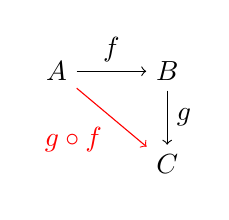
\begin{tikzpicture}[every node/.style={midway}]
\matrix[column sep={4em,between origins},
        row sep={2em}] at (0,0)
{ \node(A)   {$A$}  ; & \node(B) {$B$}; \\
                      & \node(C) {$C$}; \\};
\draw[->] (A) -- (B) node[anchor=south]  {$f$};
\draw[->] (B) -- (C) node[anchor=west]  {$g$};
\draw[->,red] (A) -- (C) node[anchor=north east] {$g\circ f$};
\end{tikzpicture}
\]
We do not really need to draw $g\circ f$ as a separate arrow because the \emph{path} from $A$ to $B$ to $C$ is already implicitly a depiction of $g\circ f$.
So the simpler diagram 
\[
\tikzset{>=stealth}
\begin{tikzpicture}[every node/.style={midway}]
\matrix[column sep={4em,between origins},
        row sep={2em}] at (0,0)
{ \node(A)   {$A$}  ; & \node(B) {$B$}; \\
                      & \node(C) {$C$}; \\};
\draw[->] (A) -- (B) node[anchor=south]  {$f$};
\draw[->] (B) -- (C) node[anchor=west]  {$g$};
\end{tikzpicture}
\]
shows the same information, namely, that $\fromto fAB$ and $\fromto gBC$ are functions and therefore, $\fromto {g\circ f}AC$ is too.

Now a diagram such as this
\[
\tikzset{>=stealth}
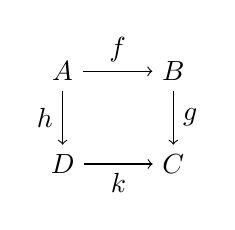
\begin{tikzpicture}[every node/.style={midway}]
\matrix[column sep={4em,between origins},
        row sep={2em}] at (0,0)
{ \node(A)   {$A$}  ; & \node(B) {$B$}; \\
  \node(D)   {$D$}  ; & \node(C) {$C$}; \\};
\draw[->] (A) -- (B) node[anchor=south]  {$f$};
\draw[->] (B) -- (C) node[anchor=west]  {$g$};
\draw[->] (A) -- (D) node[anchor=east] {$h$};
\draw[->] (D) -- (C) node[anchor=north] {$k$};
\end{tikzpicture}
\]
depicts two composite functions $g\circ f$ and $k\circ h$, but $g\circ f$ and $k\circ k$ may not be equal.
We say that the diagram \emph{commutes} or that it is a \emph{commutative diagram} if $g\circ f = k\circ h$.
In other words, saying that a certain diagram commutes \emph{is} an assertion that certain functions are equal.


\begin{exercises}
\begin{enumerate}
\item  For each of the following pairs of functions $\NN\to\NN$, determine whether they are equal and explain why or why not.
  \begin{enumerate}
  \item $f(n) = 2n + 3$ and $g(m) = 2m + 3$
  \item $f(n) = 2^{n+1} - 1$ and $g(n) = \sum_{i=0}^n2^i$
  \item $f(n) =  n^2 + 5n + 6$ and $g(n) = (n+3)(n+2)$
  \item $f(n) = n^4 - 10n^3 + 35n^2 + 50n + 24$ and $g(n) = 24$
  \end{enumerate}
\item Let $\RR$ denote the set of all real numbers. Let $f(x) = \tan(x)$.
Explain why this does \emph{not} define a function from $\RR$ to $\RR$.
\item Suppose the following functions exist: $\fromto fAB$, $\fromto gBC$, $\fromto aAD$, $\fromto bCD$. 
  Draw a commutative diagram asserting that $b\circ g\circ f = a$.
\item Suppose the following functions exist: $\fromto fCA$, $\fromto gCB$, $\fromto hCP$, $\fromto pPA$ and $\fromto qPB$.
 Draw a commutative diagram asserting that $f=p\circ h$ and $g=q\circ h$.
\end{enumerate}
\end{exercises}

\chapter{Basic Building Blocks}

\begin{goals}
	\noindent\textbf{Lecture}
	\begin{itemize}
	\item Characterize and define
		 \begin{itemize}
			 \item Pointer and constant functions
			\item Solution sets
			\item Characteristic functions
			%		 	\item The set of natural numbers
			\item Products of sets
			\item Exponents of sets
		 \end{itemize}
	\item Introduce the idea of a \emph{universal} construction.
	\end{itemize}

	\noindent\textbf{Study}
	\begin{itemize}
	\item Be able to calculate membership in various constructed sets 
	\item Learn to use universal constructions to define functions. 
	\end{itemize}
\end{goals}

So far, we have thought mainly about finite sets and a few informally defined functions on, say, the real numbers or the natural numbers.
To fill out our understanding of sets, we need to be able to build sets for specific purposes and with specific structure in mind. 

Three finite sets will play particularly important roles. We have already mentioned the set $\emptyset$, consisting of no elements.
We also need a designated set with one element and a distinguished set with two elements. We denote these by $\One$ and $\Two$. 
It does not matter at all \emph{what} elements are in these because, as we will soon see, any two sets of the same size are interchangeable.
What `interchangeable' means is discussed later.
What `same size' means is obvious for finite sets, but not at all apparent for infinite ones.
We discuss the general situation later as well.

For the time being, we merely need to agree on a fixed set with one element and a fixed set with two elements.
The particular choices I make here will be clearer as we put them to use.

\begin{defn}
	Let $\bullet$, $\bot$ and $\top$ be fixed symbols. Then define
	\begin{align*}
		\One &= \{\bullet\}\\
		\Two &= \{\bot,\top\}
	\end{align*} 
	The single element of $\One$ is intended to look like a generic point in an internal diagram.
	The element $\top$ is meant to remind you of the letter `T' (short for `True') and $\bot$ is meant to be the opposite of $\top$ (that is, 'False').
\end{defn}


\section{Elements, Pointers and Constant Functions}

Suppose we are told that $\fromto p\One A$ is a function.
Since $\bullet\in\One$, this function determines an element of $A$, namely $p(\bullet)$.
A picture of the situation might be this:
\[
  \begin{tikzpicture}[
    >=stealth,
    bullet/.style={
      fill=black,
      circle,
      minimum width=1pt,
      inner sep=1pt
    },
    projection/.style={
      ->,
      thick,
      shorten <=2pt,
      shorten >=2pt
    },
    every fit/.style={
      ellipse,
      draw,
      inner sep=0pt
    }
  ]
    \node[bullet] (p) at (0,2.5) {};

    \foreach \x/\y/\l in {4.1/1/4,3.2/2/3,4.3/3/2,4/4/1}
      \node[bullet,label=right:$\l$] (a\y) at (\x,\y) {};

    \node[draw,fit=(p),minimum width=1cm, minimum height=1cm] {} ;
    \node[draw,fit=(a1) (a2) (a3) (a4),minimum width=2cm] {} ;

    \draw[projection] (p) -- (a3);
  \end{tikzpicture}
\]
Since $\One$ has only a single element, it can ``point'' only to a single element of $A$.
So we might refer to a function $\One\to A$ as a \emph{pointer} into $A$.
Each pointer determines an element of $A$. 
And conversely, it should be possible to point to any element of $A$. 
This leads to our first (and nearly trivial) principle guaranteeing that certain functions exist.

\begin{principle}\label{ax:pointers}
	For any set $A$, and any $a\in A$, there is a function $\fromto {\hat a}\One A$ given by the rule $x\mapsto = a$.
\end{principle}

In effect, this principle simple asserts that elements of a set $A$ and functions $\One\to A$ are interchangible: from $a\in A$ we get $\fromto {\hat{a}}\One A$; from $\fromto p\One A$.
we get the element $p(\bullet)$. 

This principle also justifies the drawing of internal diagrams, like the one above, for pointers because it means that any such diagram is guaranteed to depict an actual function. 

Suppose $\fromto fA\One$ and $\fromto gA\One$ are functions, that is, their \emph{codomain} is $\One$ instead their \emph{domain}. 
Then $f(a)=g(a)$ is true for every $a\in A$ because $\bullet$ is the only possible value for $f(a)$ and $g(a)$. 
So $f=g$ by the Principle of Function Extensionality.
In other words, there is at most one function from $A$ to $\One$.
But the rule $x\mapsto \bullet$ is as simple a rule as one can imagine. 
This leads to another definition and another principle.

\begin{defn}\label{def:terminal}
	A set $T$ is \emph{terminal} if it is the case that for any set $A$ there is exactly one function from $A$ to $T$.
\end{defn}

\begin{principle}
	The set $\One$ is a terminal set. 
	We denote the unique function from $A$ to $\One$ by $\fromto {\Diamond_A}{A}\One$.
	
	The rule defining $\Diamond_A$ must be
	\[x\mapsto\bullet\]
	because no other rule is possible. 
\end{principle}

Using $\Diamond_A$ and $\hat{b}$ for an element $b\in B$, we can now define constant functions. 
That is $\hat{b}\circ\Diamond_A$ is a function from $A$ to $B$ given by the rule
$x\mapsto \hat{b}(\Diamond_A(x))$. But since $\hat{b}(\Diamond_A(x))= \hat{b}(\bullet) = b$, the rule simplifies to $x\mapsto b$. 
In short, this is the function sending any element of $A$ to the constant result $b$. 

\begin{exercises}
	\begin{enumerate}
		\item Show that for any pointer $\fromto p\One A$, it is the case that $\widehat{p(\bullet)}=p$.
		\item Show that any set with exactly one element is a terminal set.
		\item Suppose that $\fromto fAB$ is a function. Show that for every $a\in A$, $\widehat{f(a)} = f\circ \hat{a}$.
	\end{enumerate}
\end{exercises}

\section{The Empty Set}

For trivial reasons, there is at most one function from $\emptyset$ to $A$,
for any set $A$. That is,  if $\fromto {f,g}\emptyset A$ are functions, then
for each $x\in\emptyset$, $f(x)=g(x)$ because there are no $x$'s to concern us. Hence by Principle \ref{ax:FunctionExtensionality}, $f=g$. The empty ``rule'' that tells us nothing does actually specify a function from $\emptyset$ to $A$. So for any set $A$, there is exactly one function from $\emptyset$ to $A$.

\begin{defn}
	An \emph{initial set} is a set $I$ so that for any set $A$, there is exactly one function from $I$ to $A$.
\end{defn}

\begin{principle}
	The emptyset $\emptyset$ is an initial set. For a set $A$, the unique
	function from $\emptyset$ to $A$ may be denoted by 
	$\fromto {\Box_A}\emptyset A$.
\end{principle}

Notice that a function $A\to\emptyset$ is impossible unless $A$ is also empty.
So it follows that $\emptyset$ is the only initial set. 

\begin{exercises}
	\begin{enumerate}
		\item How many functions are there from $\emptyset$ to $\{a,b,c,d\}$? Explain.
		\item How many functions are there from $\{a,b,c,d\}$ to $emptyset$? Explain.
		\item How many functions are there from $\One$ to $\{a,b,c,d\}$? Explain.
		\item How many functions are there from $\{a,b,c,d\}$ to $\One$? Explain.
	\end{enumerate}
\end{exercises}

\section{Solution Sets, Subsets, Characteristic Functions}

Suppose we are given two functions that are ``parallel'': $\fromto fAB$ and $\fromto gAB$.
Then for some value $a\in A$, it might be the case that $f(a)=g(a)$.
We may call such a value a \emph{particular solution to the equation $f(x)=g(x)$}. 
It might be the case that there are no particular solutions.
For example, there are no natural numbers $n$ such that $n+1 = n$. 
On the other hand, there might be many particular solutions. 
For example, let $f(x)=x^3$ and let $g(x)= 6x^2 - 11x + 6$ both regarded as functions on the natural numbers.
Then it is easy to check that $1$, $2$ and $3$ solve the equation $f(x)=g(x)$.
In fact, these three are the only particular solutions.
We generalize as follows.

\begin{defn}\label{def:equalizer} 
	For two functions $A\doublerightarrow{f}{g} B$, a \emph{solution} is a function $\fromto sCA$ so that 
	\[f\circ s = g\circ s.\]
	Thus for example, if $a\in A$ is a particular solution then the pointer $\hat a$ is a solution. 

	For functions $A\doublerightarrow{f}{g} B$, an \emph{equalizer} is solution $\fromto eEA$ so that for any solution $\fromto sCA$, there is exactly one function $\fromto hCE$ so that \[e\circ h = k.\]
\end{defn}

\begin{principle}
	For functions $A\doublerightarrow{f}{g} B$, the collection of all particular solutions to the equation $f(x)=g(x)$ form a set, denoted by $\{x\in A\st f(x) = g(x)\}$. 	
	The function $\fromto i{\{x\in A\st f(x)=g(x)\}}A$ given by the rule $x\mapsto x$ (called an \emph{inclusion map}) is an equalizer for $f$ and $g$.
	
	If $\fromto sCA$ is a solution of  $f(x)=g(x)$, that is, $f\circ s = g\circ s$,
	then the function $\fromto {\check s}C{\{x\in A\st f(x)=g(x)\}}$ given by the rule $x\mapsto s(x)$
	is the unique function for which $s = i\circ \check s$. 
\end{principle}

This axiom tells us three main things.
First, we can form a subset of $A$ by specifying an equation $f(x)=g(x)$ for any two functions $A\doublerightarrow{f}{g}B$, and picking out the particular solutions.
Second, a subset formed in this way ``embeds'' in the given set $A$ by its inclusion map $i$.
Third, for any solution $s$, the function into the set of particular solutions is defined by the same rule as $s$.

Suppose $c\in C$ and $\fromto fAC$ is a function, then we can form the equalizer of $f$ and the constant function $\hat{c}\circ\Diamond_A$.
This is more easily written we $\{x\in A\st f(x)=c\}$.
Since it common to pick out sets like this, special notation is in order.

\begin{defn}\label{def:inverse-image}
	For a function $\fromto fAC$, and a value $c\in C$, 
	\[f^-(c) = \{x\in A\st f(x)=c\}.\] 
	In this case, $f^-(c)$ is called the \emph{inverse image of $c$ with respect to $f$}.
\end{defn}

Evidently, in Definition \ref{def:inverse-image}, the set $f^-(c)$ is a subset of $A$.
It would be good to know that any subset of $A$ can be described as an inverse image.
This is where the set $\Two$ plays a role.

\begin{defn}\label{def:subset-classifier}
	A \emph{subset classifier} is a set $S$ with a distinguished element $t\in S$ so that for any set $A$ and any subset $B\subseteq A$, there is exactly one function $\fromto kAT$ for which $B = k^-(t)$.
	That is, $B$ is uniquely defined as the inverse image of $t$ with respect to a function into $S$.
\end{defn}

\begin{principle}\label{ax:subset-char}
	The set $\Two$ with the distinguished element $\top$ is a subset classifier.
	For subset $B\subseteq A$, the function corresponding to $B$, called the \emph{characteristic function of $B$}, is denoted by $\kappa_B$.
	In other words, $\kappa_B$ is the unique function for which $B = \kappa_B^-(\top)$.

	For $B\subseteq A$, the characteristic function is defined by the rule
	\[
	x \mapsto
		\begin{cases}
			\top &\text{ if } x\in B\\
			\bot &\text{ otherwise}
		\end{cases}
	\]
\end{principle}

Just as Principle \ref{ax:pointers} asserts that elements of $A$ and functions $\One\to A$ are interchangeable, Principle \ref{ax:subset-char} asserts that the subsets of $A$ and the functions $A\to\Two$ are interchangeable.

\begin{exercises}
	\begin{enumerate}
	\item Draw a depiction of $A=\{a,b,c,d,e,f,g\}$ and its subset $B=\{a,c,e,g\}$ in the same internal diagram. Now depict the characteristic map for $B$ as a subset of $A$.
	
	\item Define two functions $\NN\doublerightarrow{f}{g}\NN$ so that the set of particular solutions fo $f(x)=g(x)$ is $\{1,5\}$. 
	
	\item Consider the functions $\fromto f\RR\RR$ defined by $f(x) = \sin(x) + \cos(x)$, and $\fromto s\NN\RR$ defined by $s(n) = 2\pi n^2$. 
	Is $s$ a solution for the equation $f(x) = -1$? 
	What is the set of all particular solutions?
	\end{enumerate}
		
\end{exercises}

\section{Product Sets and Functions of Two Arguments}

We should be able to deal with functions of more than one argument, such as a function $f(x,y) = x+y$.
To account for these, we take our cue from Descartes.

Descartes studied the geometric plane in terms of a coordinate system consisting of the so-called $x$-axis and $y$-axis (what we call cartesian coordinates in his honor).
Once we have decided where to place the axes (as long as they do not run in parallel), a pair such as $(2,3)$ determines a point on the plane, and any point $p$ in the plane determines a pair.
So Descartes realized that we might as well just say that the plane actually \emph{is} the collection of all pairs of real numbers.
What makes this work is that points in the plane \emph{project} onto the two axes in a universal way.
Products of sets generalize this idea.

\begin{defn}
For sets $A$ and $B$, a \emph{table} consists of two functions $A\stackrel{f}{\longleftarrow} C\stackrel{g}{\longrightarrow}B$.
Note that the two functions have the same domain. We may call the two functions \emph{legs} of the table.

For sets $A$ and $B$, a \emph{product of $A$ and $B$} is a table $A\stackrel{p}{\longleftarrow} P\stackrel{q}{\longrightarrow}B$ so that for any table $A\stackrel{f}{\longleftarrow} C\stackrel{g}{\longrightarrow}B$ there is exactly one function $\fromto hCP$ for which $f = p\circ h$ and $g= q\circ h$. 
For a product, the legs $p$ and $q$ are called the \emph{projections}.
\end{defn}

\begin{principle}\label{ax:products}
	For sets $A$ and $B$, the collection of all pairs $(a,b)$ where $a\in A$ and $b\in B$ is a set, denoted by $A\times B$. 
	The functions $A\stackrel{\pi_0}{\longleftarrow}{A\times B}\stackrel{\pi_1}{\longrightarrow}B$ given by the rules $(a,b)\mapsto a$
	and $(a,b)\mapsto b$ are projections. For $A\stackrel{f}{\longleftarrow}{C}\stackrel{g}{\longrightarrow}B$, the unique function required by
	the product may be denoted by $\langle f,g\rangle$.

	For $A\stackrel{f}{\longleftarrow}{C}\stackrel{g}{\longrightarrow}B$, the function $\fromto {\langle f,g\rangle}C{A\times B}$ is defined by the rule $\langle f,g\rangle(x)=(f(x),g(x))$.
\end{principle}

Suppose we are given two unrelated functions $\fromto fAB$ and $\fromto gCD$. 
We can now form a single function from $A\times C$ to $B\times D$ by combining $f$ and $g$ ``independently''. 
That is, define $f\times g = \langle f\circ \pi_0,g\circ \pi_1\rangle$.
Calculating concretely in terms of elements $(f\times g)(x,y) = (f(x),g(y))$. 
So $f\times g$ acts on a pair $(x,y)$ by applying $f$ to $x$ and unrelatedly applying $g$ to $y$. 

Products can by generalized to three, four or more sets.
For example, for sets $A$, $B$ and $C$, we might write $A\times B\times C$ for the set of triples $(a,b,c)$ where $a\in A$, $b\in B$ and $c\in C$. 
Instead of two projections, this would have three projections $(x,y,z)\mapsto x$, and so on. 
It turns out, however, that binary products are enough because $A\times (B\times C)$ behaves just like $A\times B\times C$.

\begin{exercises}
	\begin{enumerate}
		\item For the sets $A = \{a,b,c\}$ and $B = \{1,2,3,4\}$, calculate $A\times B$ and $B\times A$
		\item What is $\emptyset \times A$? 
		\item Calculate $\{4,a,0\}\times \Two$.
		\item Describe in plain English what are the elements of $\NN\times \NN$.
		\item Suppose $A$ is a finite set with $m$ elements and $B$ is a finite set with $n$ elements.
		How many elements are in $A\times B$?
		Describe in plain English why it makes sense to refer to $A\times B$ as a ``product.''
		\item For sets $A=\{a,b\}$, $B=\{0,1,2\}$ and $C=\{c,d\}$, calculate $A\times B\times C$, $A\times (B\times C)$ and $(A\times B)\times C$.
		\item Define the standard fifty-two card poker deck as a product of two sets.
	\end{enumerate}
\end{exercises}

\section{Function Sets}

A function from $A$ to $B$ might depend on a parameter from $C$. 
For example, the function $\fromto f\RR\RR$ defined by the rule $f(x) = \sin(x + c)$ depends on the constant $c$.
There is a related function $\fromto g{\RR\times \RR}\RR$ defined by $g(c,x) = \sin(x+c)$.
Evidently, $g$ describes the same behavior as $f$, but it makes the parameter explicit. It will be helpful to relate $g$ -- a function on pairs -- to $f$ a function with a parameter.
This leads to the following definition.

\begin{defn}
	For sets $A$ and $B$, a \emph{parametric function from $A$ to $B$} is a function $\fromto g{C\times A}B$ for some set $C$.
	The set $C$ may be called the \emph{set of parameters}.
	
	Suppose $\fromto f{D\times A}B$ is a parametric function with parameter set $D$ and $\fromto kCD$ is a function.
	Then we can form another parametric function with parameters in $C$ by composition: $f\circ (k\times \id_A)$.
	We may refer to $k$ as a \emph{change of parameters} function because $k$ transforms the parametric function with parameters in $D$ into a parametric function with parameters in $C$. 
	Specifically, $f\circ(k\times \id_A)$ is given by the rule $(c,a)\mapsto f(k(c),a)$. 
	
	An \emph{evaluation map} for $A$ and $B$ is a parametric function $\fromto a{F\times A}B$, so that for any 
	parametric function $\fromto g{C\times A}B$ there is exactly one change of parameters $\fromto hCF$ so that
	$g = a\circ (h\times \id_A)$. In that case, $F$ is called an \emph{exponential with base $B$ and exponent $A$}.
\end{defn}

\begin{principle}
	For sets $A$ and $B$, the collection of all functions from $A$ to $B$, denoted by $B^A$, is a set.
	Moreover, there is an evaluation map $\fromto \appl{B^A\times A}B$ defined by the rule $(f,x) \mapsto f(x)$.
	The unique change of parameters function corresponding to $\fromto f{C\times A}B$ does not have a completely standard name.
	Some mathematicians honor the twentieth century logician, Haskell Curry, by referring to this as `currying'.
	For these lectures, we follow that tradition and write $\curry[f]$ for the unique function satisfying $f = \appl\circ (\curry[f] \times \id_A)$.
	
	Calculating how $\fromto {\curry[f]}C{B^A}$ must behave, we see that $\curry[f](c)$ is the function from $A$ to $B$ given by the rule $x\mapsto f(c,x)$.
	So for any $c\in C$, $\curry[f](c)$ is the function such that for any $a\in A$, $\curry[f](c)(a) = f(c,a)$. 
\end{principle}

\subsection*{$\lambda$ Notation}

When we describe a function by a rule like $x\mapsto x^2$, it is usually convenient to give the function a name.
So we might write $f(x) = x^2$.
But sometimes, it is also convenient to have a notation for a function without giving it an explicit name. 
The logician Alonzo Church \cite{church} proposed a simple notation to describe functions. 
He wrote things like $\lambda x.x^2$ to describe the function that squares its input. 
The Greek letter $\lambda$ is used merely as a marker to introduce a function. 
It does not mean anything special. 
We could make the $\lambda$ notation formal, but for our purposes we do not need that.

\begin{example}
	Suppose $\fromto fAB$ and $\fromto gBC$. Then $g\circ f$ is the function
	$\lambda x.g(f(x))$.  So $f\in B^A$ and $g\in C^B$ determine $g\circ f\in C^A$.
	Thus $\circ$ can be regarded (locally) as a function $B^A\times C^B\to C^A$.
	It is defined by $\lambda(f,g).\lambda x.g(f(x))$.
\end{example}
 

\begin{exercises}
	\begin{enumerate}
		\item  For set $A= \{1,2,3\}$ and $B = \{a,b\}$ 
			\begin{enumerate}
				\item draw internal diagrams corresponding to each element of $B^A$ (there are eight of them);
				\item draw internal diagrams corresponding to each element of $A^B$ (there are nine of them).
			\end{enumerate}
		\item Consider the function $\fromto f{\NN\to\NN}\NN$ defined by
		      $f(m,n) = m^n$. What function is $\curry[f](3)$? Use $\lambda$ notation to describe it.
	\end{enumerate}	
\end{exercises}

\section{Universal Constructions}

Consider the product $A\times B$ again.
It possesses functions 
$A\stackrel{\pi_0}{\longleftarrow}A\times B\stackrel{\pi_1}{\longrightarrow}B$. For any other similar arrangement
$A\stackrel{f}{\longleftarrow}C\stackrel{g}{\longrightarrow}B$, there is a unique function $C\stackrel{\langle f,g\rangle}{\longrightarrow}{A\times B}$ making the diagram
\[
\tikzset{>=stealth}
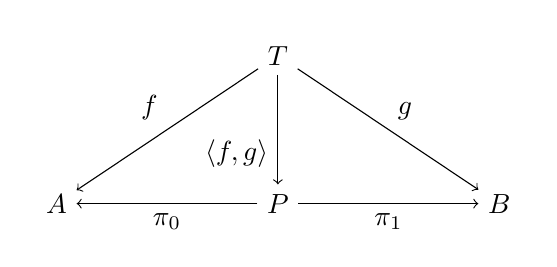
\begin{tikzpicture}[every node/.style={midway}]
\matrix[column sep={4em,between origins},row sep={2em}] at (0,0)
{ 					&	& \node(T) {$T$}; &	& \\
	\\
	\node(A)   {$A$}; &	& \node(P) {$P$}; &	& \node(B) {$B$}; \\};
\draw[->] (T) -- (A) node[anchor=south east]  {$f$};
\draw[->] (T) -- (B) node[anchor=south west]  {$g$};
\draw[->] (T) -- (P) node[anchor=north east] {$\langle f,g \rangle$};
\draw[->] (P) -- (A) node[anchor=north] {$\pi_0$};
\draw[->] (P) -- (B) node[anchor=north] {$\pi_1$};
\end{tikzpicture}
\]
commute.

An equalizer ($\{x\in A\st f(x)=g(x)\}$), a terminal object ($\One$) and an exponential ($B^A$) are also characterized by some special functions so that any similarly arranged functions determine a unique function making a suitable diagram commute.
Go back and reread the definitions of equalizers, terminal objects, products and exponentials to see that they all have this family resemblance.
They are called \emph{universal constructions}.
So the inclusion $\{x\in A\st f(x)=g(x)\}\to A$ is universal for solving the equation $f=g$; $A\stackrel{\pi_0}{\longleftarrow}A\times B\stackrel{\pi_1}{\longrightarrow}B$ is universal for mapping into $A$ and $B$;
$B^A\times A\stackrel{\appl}B$ is the universal parametric function from $A$ to $B$.
The principles of this lecture spell out that there are sets and functions 
with the desired universal properties.

\begin{exercises}
	\begin{enumerate}
		\item Explain how $\One\stackrel{\hat{\top}}{\longrightarrow}\Two$ is universal. [There is not a single intended correct answer to this. 
		I want you to think about how $\Two$ fits into a bigger picture.]
	\end{enumerate}
\end{exercises}

\section{Relations and Function Graphs}

We have already noted that a chaacteristic function $\fromto R{X\times Y}\Two$ corresponds to a subset of $X\times Y$. We can think of $R$ \emph{relating} elements of $X$ to elements of $Y$. This leads to a useful definition.

\begin{defn}
	A \emph{relation from $X$ to $Y$} is a function $\fromto R{X\times Y}\Two$.
	A \emph{relation on $X$} is a relation from $X$ to $X$.
	
	For a relation $R$ from $X$ to $Y$, we will say ``$x$ is $R$-related to $y$'' and write $R(x,y)$ when $R(x,y)=\top$. In some situations, we may use ``infix'' notation, writing $x\mathrel{R}y$ instead of $R(x,y)$.
	
	A relation $\fromto R{X\times Y}\Two$ is
	\begin{itemize}
		\item \emph{total} if for every $x\in X$, there is at least one $y\in Y$ for which $x\mathrel{R}y$;
		\item \emph{deterministic} if for every $x\in X$, there is at most one $y\in Y$ for which $x\mathrel{R}y$;
		\item \emph{functional} if it is total and deterministic.
	\end{itemize}
\end{defn}

\begin{example}
	The relation of $\leq$ on real numbers can be regarded as a function $\fromto {\mathord{\leq}}{\RR\times\RR}{\Two}$ defined by $\mathord\leq(x,y) = \top$ when $x$ is actually less than or equal to $y$ and $\mathord\leq(x,y)=\bot$ otherwise. This is a good example of why we prefer to write $x\leq y$ instead of $\mathord\leq(x,y)$ or $\mathord\leq(x,y)=\top$.

	The relation $=$ on any set is functional because, for any $x\in X$ there is exactly one $y\in X$ so that $x=y$. 
\end{example}

\begin{defn}
A function $\fromto fXY$ determines a relation called the \emph{graph of $f$} defined by 
\[\Gamma_f(x,y) = \begin{cases}
					\top &\text{if $f(x)=y$}\\
					\bot &\text{otherwise}
				\end{cases}.
\]
\end{defn}

\begin{lemma}
	For any function $\fromto fYX$, the graph $\Gamma_f$ is functional.
	
	\begin{proof}
		This is pretty obvious from the basic properties of functions. That is,
		for each $x\in X$, $f(x)\in Y$ and obviously $f(x)=f(x)$. So $\Gamma_f$ is total. On the other hand if $y = f(x)$ and $y'=f(x)$, then $y=y'$. So $\Gamma_f$ is deterministic.
	\end{proof}
\end{lemma}

But suppose we have a functional relation $\fromto R{X\times Y}\Two$. Then it is reasonable to suppose it actually came from a function.

\begin{principle}\label{princ:graphs}
	Suppose $\fromto R{X\times Y}{\Two}$ is a functional relation. Then there is a function $\fromto {F_R}XY$ so that $\Gamma_{F_R} = R$.
\end{principle}

It is easy enough to check that $F_{\Gamma_f} = f$ for any function $f$. That is,
$F_{\Gamma_f}(x)=y$ if and only if $x\mathrel{\Gamma_f} y$ if and only if $f(x)=y$. So functions from $X$ to $Y$ correspond exactly to functional relations
from $X$ to $Y$. 

\chapter{The Set of Natural Numbers}\label{lec:natural-numbers}

\begin{goals}
\noindent\textbf{Lecture:}
\begin{itemize}
	\item Re-introduce the natural numbers as a set
	\item Introduce sequences and recursively defined sequences
	\item Relate recursion to proofs by induction
\end{itemize}

\noindent\textbf{Study:}
\begin{itemize}
	\item Be able to define simple functions by recursion
	\item Be able to prove explain how induction and recursion are related
\end{itemize}
\end{goals}

We have used $\NN$ informally to denote the set of natural numbers. 
It is time that we make the structure of $\NN$ explicit within our theory of sets and functions. 
It will turn out that $\NN$ is also a universal construction. 

Natural numbers provide a precise picture of counting and of putting things in an order: first, second, third, and so on.
Now that we have sets and functions we can consider a function $\fromto a\NN A$ to be an \emph{infinite sequence}: $a(0)$, $a(1)$, $a(2)$, \ldots.
When we do that, we sometimes write $a_0$, $a_1$, $a_2$, \ldots instead. Still $a$ itself is just function from $\NN$ to $A$. To emphasize the notation that 
$a$ represents an infinite sequence, we sometimes also write $(a_i)_{i\in I}$.

Much of what we discuss in this lecture has about it the feel of computer programming.
This is partly because natural numbers are the main objects of calculation.
We want to understand, for example, how to define a function like $n\mapsto n!$ ($n$ factorial) as a function from $\NN$ to $\NN$ by specifying how it behaves.
In particular, $0! = 1$ and $(n^\nxt)! = n^\nxt\cdot n!$ characterize factorial by spelling out how to calculate it.
For example,
\begin{align*}
	4!  &= 4 \cdot 3! \\
		&= 4 \cdot (3 \cdot 2!)\\
		&= 4 \cdot (3 \cdot (2 \cdot 1!))\\
		&= 4 \cdot (3 \cdot (2 \cdot (1 \cdot 0!)))\\
		&= 4 \cdot (3 \cdot (2 \cdot (1 \cdot 1)))
		&= 24
\end{align*}

It is quite common to think about a sequence in which $a_{n+1}$ is functionally related to $a_n$. 
For example, in the sequence $1, 2, 4, 8,\ldots$, the initial entry is $1$ and each successive entry is double its predecessor.

Indeed, if we know just those two facts -- the initial entry is $1$, and each subsequent entry is double its predecessor -- then we know how the entire sequence behaves.
Also, we know how to calculate the $n^{\text{th}}$ entry, by recursion just like factorial.

The most basic sequence, of course, is $0$, $1$, $2$, \ldots. 
Its initial entry is $0$ and each subsequent entry is the successor of its predecessor. 
So we think of the sequence that comprises $\NN$ as a universal recursively defined sequence.

\section{Sequences and Simple Recurrences}

Let us make the informal word \emph{sequence} official.

\begin{defn}
	A \emph{sequence in $A$} is a function $\fromto a\NN A$.
\end{defn}

As we studied in previous lectures, the basic vocabulary of natural numbers is that (i) there is a starting natural number $0$ and (ii) for each natural number $n$ there is a next one, $n^\nxt$. 
To discuss successor in the language of sets and functions, we can stipulate that successor is a function $\fromto \suc\NN\NN$ given by the rule $n\mapsto n^\nxt$.
So $\NN$ is not only a set. 
It comes with functions $\One \stackrel{\hat{0}}{\longrightarrow} \NN \stackrel{\suc}{\longleftarrow} \NN$.

Suppose $\One\stackrel{\hat{b}}{\longrightarrow}A\stackrel{r}{\longleftarrow}A$ is a similar structure.
Then we ought to be able to define a sequence in $A$, so that $a_0=b$, $a_1=r(b)$, $a_2=r(r(b))$, and so on. 
In general, $a_k$ should be determined by starting with $b$ and repeatedly applying $r$ a total of $k$ times. 

\begin{defn}\label{def:nno}
	A \emph{simple recurrence} is a set with functions $\One\stackrel{\hat{b}}{\longrightarrow}C\stackrel{r}{\longleftarrow}C$.
	
	A \emph{countably infinite set} is a simple recurrence $\One\stackrel{\hat{z}}{\longrightarrow}N\stackrel{s}{\longleftarrow}N$ so that for any other simple recurrence $\One\stackrel{\hat{b}}{\longrightarrow}C\stackrel{r}{\longleftarrow}C$, there is exactly one function $\fromto fNC$ so that $f\circ \hat{z} =\hat b$ and $f\circ s = r\circ f$.
	
	Simple recurrences go by lots of other names in the literature. You will recognize them later when you see them.
\end{defn}

The principle we are interested in here is that simple recurrences determine sequences. In the next section, we discuss why we have called these ``simple''.

\begin{principle}\label{ax:nat-numbers}
	The collection of natural numbers is a set, denoted by $\NN$.
	Moreover, $\One \stackrel{\hat{0}}{\longrightarrow} \NN \stackrel{\suc}{\longleftarrow} \NN$.
	makes $\NN$ a countably infinite set.
	
	From a simple recurrence $\One \stackrel{\hat{b}}{\longrightarrow} C \stackrel{r}{\longleftarrow} C$, the corresponding unique sequence in $C$
	may be denoted by $\rec[b,r]$. So $\fromto {\rec[b,r]}\NN A$ is characterized by
	\begin{align*}
		\rec[b,r]_0 &= b\\
		\rec[b,r]_{n^\nxt} &= r(\rec[b,r]_n)
	\end{align*}
\end{principle}

Thus every simple recurrence in $C$ determines a sequence in $C$. 
On the other hand, it is not the case that every sequence is determined by a simple recurrence.
Take for example, the sequence $0,1,0,2,0,3,\ldots$. 
This can not be defined by giving an initial entry ($0$) and specifying successive entries based only on the predecessors. 
After all, the entries $1$, $2$, $3$ and so on all have the same preceding entry.

\section{Primitive Recursion}

Evidently, addition, multiplication, factorial, and other familiar functions should be definable using Principle \ref{ax:nat-numbers}. 
But there are problems to overcome: Addition is not a sequence, at least not in an obvious way. And factorial is not obviously definable by a simple recurrence
because we would need a function $\fromto r\NN\NN$ so that $n^\nxt! = r(n!)$
for all $n$. If, in place of $r$, we could use a function that depends on $n$ as well as on $n!$, we could define factorial recursively the usual way.

Putting things together, we consider a scheme that generalizes simple recursion to permit (i) dependence on $n$ at each stage of the recursion and (ii) dependence on a parameter not explicitly involved in the recursion.

\begin{defn}
	A \emph{primitive recurrence in $A$ (with parameters in $C$)} consists of two  functions $C\stackrel{b}{\longrightarrow} A\stackrel{r}{\longleftarrow}\NN\times C\times A$.
	
	A \emph{parametric sequence in $A$ with parameters in $C$} is a function
	$\fromto a{C\times \NN}A$. For a parametric sequence, we may write $a_{c,n}$
	instead of $a(c,n)$. 
\end{defn}

\begin{lemma}
	For any primitive recurrence $C \stackrel{b}{\longrightarrow} A \stackrel{r}{\longleftarrow} C\times \NN \times A$, there is a unique
	function $\fromto f{C\times \NN}A$ satisfying: 
	\begin{align*}
		f_{c,0} &= b(c)\\
		f_{c,k^\nxt} &= r(c,k,f_{c,k})
	\end{align*}

	\begin{proof}
		The proof of this is intricate enough that we do not have room to give all the details here. 
		
		The idea of the proof is to use simple recursion to define a sequence of binary relations $R_0$, $R_1$, \ldots, from $C\times \NN$ to $A$. In other words, $R$ is a function from $\NN$ to $\Two^{(C\times \NN)\times A}$. 
		These relations will satisfy the following conditions for each $i\in\NN$:
		\begin{itemize}
			\item $R_i\subseteq R_{i^\nxt}$;
			\item $R_i$ is deterministic;
			\item $R_i$ is total on $\{0,\ldots, i-1\}$
		\end{itemize}
		Then we define $R$ to be the relation $(c,n)\mathrel{R}a$ if and only if $(c,n)R_i a$ holds for some $i\in \NN$. 
		It follows from the above conditions that $R$ is functional. So there is a function $\fromto f{C\times\NN}A$ for which $f(c,n)=a$ if and only if $(c,n)\mathrel{R}a$. By the construction of $R$, it will follow that $f$ satisfies  
		\begin{align*}
			f_{c,0} &= b(c)\\
			f_{c,k^\nxt} &= r(c,k,f_{c,k})
		\end{align*}
			
		Define $R_0$ to be the constantly $\bot$ relation. 
		This is clearly deterministic and since $C\times \emptyset = \emptyset$, it is total on that set.
		Define $\fromto p{\Two^{(C\times\NN)\times A}}{\Two^{(C\times \NN)\times A}}$ by the following rules (writing $p_R$ for $p(R)$ to eliminate some confusing parentheses:
		\begin{itemize}
			\item $(c,0)\mathrel{p_R}b(c)$
			\item $(c,k^\nxt)\mathrel{p_R}x$ if and only if either
			 \begin{itemize}
			 	\item $(c,k^\nxt)\mathrel{R}x$ or
			 	\item for some $y$, $(c,k)\mathrel{R}y$ and $r(c,k,y)=x$.
			 \end{itemize}
		\end{itemize}
		Now we check that (i) $R\subseteq p_R$, (ii) if $R$ is deterministic then $p_R$ is deterministic, and (iii) if $R$ is total on $C\times \{0,\ldots, k-1\}$, then $p_R$ is total on $C\times \{0,\ldots,k\}$. 
		Consequently, defining $R_i$ by the simple recurrence $\rec[R_0,p]$, we can prove by induction that the conditions stated in the second paragraph hold. 
		Finally, by the way we constructed $R$, $f_{c,o} = b(c)$  and by induction on $k$, $f_{c,k^\nxt} = r(c,k,f_{c,k})$. 
	\end{proof}
\end{lemma}

\newcommand{\pred}{\mathord{\textsf{pred}}}
\begin{example}
	The ``predecessor'' function is defined by the scheme $\pred(0)=0$ and $\pred(n^\nxt) = n$. 
	The primitive recurrence
	$\One \stackrel{\hat0}{\longrightarrow} \NN \stackrel{\pi_2}{\longleftarrow} \One\times\NN\times\NN$ where $\pi_1$ is the projection $(x,y,z)\mapsto y$ determines a function $\fromto g{\One\times \NN}{\NN}$ given by
	$g_{\bullet, 0} = 0$ and $g_{\bullet,n^\nxt} = \pi_2(\bullet, n, g_{\bullet, n}) = n$. Hence, we may define $\pred(n) = g_{\bullet, n}$
\end{example}



\begin{exercises}
\begin{enumerate}
	\item For a given function $\fromto f\NN\NN$, find a primitive recurrence that defines the function $n\mapsto \sum_{i=0}^{n-1}f(i)$. That is, result will be the sequence $0$, $f(0)$, $f(0)+f(1)$, $f(0)+f(1)+f(2)$, \ldots.
	\item Find a primitive recurrence that defines the function from $\NN\times \NN$ to $\NN$ given by the rule $(m,n)\mapsto m^n$.
	\item Define the operation of \emph{monus} $m\stackrel{.}{-} n$ to be $m-n$ when $m \geq n$ and to be $0$ otherwise by  a primitive recurrence.
	\item Define the function $\lambda(m,n).m^n$ by primitive recursion.
\end{enumerate}
\end{exercises}

\section{Lists}

For a set $A$, the lists of elements from $A$ also should form a set.
The structure of this set is similar to $\NN$.

\begin{defn}
	For a set $A$, a \emph{simple $A$ recurrrence} is two functions
	$\One \stackrel{\hat b}{\longrightarrow} C \stackrel{r}{\longleftarrow} A\times C$.
	
	For a set $A$, an \emph{$A$-list set} is a simple $A$ recurrence 
	$\One \stackrel{\hat{e}}{\longrightarrow} L \stackrel{c}{\longleftarrow} A\times L$ so that for any simple $A$ recurrence $\One \stackrel{\hat b}{\longrightarrow} C \stackrel{r}{\longleftarrow} A\times C$ there is exactly one function $\fromto hLC$ so that 
	\begin{align*}
		h\circ \hat e 	&= \hat b\\
		h\circ c 		&= r\circ (\id_A\times h).
	\end{align*}
\end{defn}

\begin{principle}
	The collection of lists with items in $A$ is a set, denote by $\List[A]$.
	The functions $\fromto {\widehat{[\,]}}\One{\List[A]}$ and $\fromto c{A\times\List[A]}{\List[A]}$ defined by the rule $(a,L)\mapsto a:L$,
	constitute an $A$-list set.
	
	For $\One \stackrel{\hat b}{\longrightarrow} C \stackrel{r}{\longleftarrow} A\times C$, we may our notation for recursive functions defined from $\NN$
	and write $\rec[\hat b,r]$ for the unique function 
	satisfying $\rec[\hat b,r]([\,])= b$
	and $\rec[\hat b,r](a:L)= r(a, \rec[hat b, L](L))$.  
\end{principle}

\begin{example}
	$\One \stackrel{\hat 0}{\longrightarrow} \NN \stackrel{+}{\longleftarrow} \NN\times \NN$ determine a function $\rec[\hat 0, +]$ from $\List(\NN)$ to $\NN$. The function satifies $\rec[\hat 0,+]([\,])= 0$ and $\rec[\hat 0,+](n:L)= n + s(L)$.
	So $\rec[0,+]$ returns the sum of items of a list natural numbers.
	Earlier, we wrote this as $\sum L$.
\end{example}


\begin{exercises}
	\begin{enumerate}
		\item For a function $\fromto fAB$, specify a simple $A$ recurrence that defines the function
			\[\fromto {\map[f]}{\List[A]}{\List[B]}\] so that \[\map[f]([a_0,a_1,\ldots, a_{n-1}]) = [f(a_0),f(a_1),\ldots, f(a_{n-1})]\]
		\item Define concatenation in $\List[A]$ by a simple $A$ recurrence. [Hint: I am asking for a function from $\List[A]\times \List[A]$ to $\List[A]$, but simple $A$ recurrence alone will not do it, because that can only define a function $\List[A]\to C$ for some  $C$. Do this instead: (i) specify a simple $A$ recurrence to define a function $\fromto c{\List[A]}{\List[A]^{\List[A]}}$ for which $c(M)(L)$ is the concatetation of $L$ followed by $M$, (ii) Now define $L\star M$ to be $c(L)(M)$.
		\item Write a scheme for ``primitive $A$ recursion''. Specified by a function $\fromto bPC$ and a function $\fromto r{P\times A\times \List[A] \times C}C$,
		write equations involving $b$ and $r$ that should determine a unique function $P\times \List[A]\to C$. 
	\end{enumerate}
\end{exercises}

\chapter{Powersets}

The exponential $\Two^A$ for any set $A$ is the set of all characteristic maps on $A$.
Each element $k\in \Two^A$ corresponds to a subset of $A$ by $k^{-1}(\top) = \{x\in A\st k(x)=\top\}$. Vice versa, a subset $A\subseteq X$ determines a characteristic function $\fromto {\kappa_A}X\Two$ by the rule
\[x\mapsto \begin{cases}
			\top &\text{if $x\in A$}\\
			\bot &\text{otherwise}
\end{cases}
\]
So $\Two^X$ is, in a sense, \emph{representative} of the collection of all subsets of $X$. 
It is convenient also to suppose that the actual collection of subsets of a set $A$ forms a set.
This should ``behave'' exactly like $\Two^A$, but concretely, it consists of sets rather than characteristic functions.

\begin{principle}\label{ax:powerset}
	For any set $A$, the collection of subsets of $A$ is a set, denoted by $\powerset(A)$, and called the \emph{power set of $A$}. Moreover, there is a function $\fromto {\ni_A}{\powerset(A)\times A}\Two$ defined by 
	\[\ni_A(B,x) = \begin{cases}
	\top, &\text{ if } x\in B\\
	\bot &\text{otherwise}
	\end{cases}
	\]
	The function $\ni_A$ is an evaluation map, meaning that 
	for any function $\fromto f{C\times A}\Two$, there is a unique function $\fromto {\overline{f}}C{\powerset(A)}$ for which $f = \ni_A\circ (\overline{f} \times \id_A)$. The function $\overline f$ 
	is given by the rule $c\mapsto \{x\in A\st f(c,x)=\top\}$.
\end{principle}

For a function $\fromto fAB$, $\ni_B\circ (\id_{\powerset(B)}\times f)$ is a function from $\powerset(B)\times A$ to $\Two$. So there is a unique function
from $\powerset(B)$ to $\powerset(A)$ determined by $f$. 

\begin{defn}
	For $\fromto fAB$, let $\fromto {f^{-1}}{\powerset(B)}{\powerset(A)}$ denote
	the unique function for which $\ni_B\circ (\id_{\powerset(B)}\times f) = \ni_A\circ(f^{-1}\times \id_A)$. In simpler terms, $f^{-1}$ satsifies
	\[x\in f^{-1}(Y) \text{if and only if } f(x)\in Y\]
	for every $Y\subseteq B$.  So $f^{-1}$ is given by the rule $Y\mapsto \{x\in A\st f(x)\in Y\}$
\end{defn}

This notation does not clash much with our earlier definition of inverse image of an element, $f^{-1}(b)$, because 
$f^{-1}(b)$ (from the earlier usage) is the same as $f^{-1}(\{b\})$.

\section{Intersections, Unions, Residuals, Differences and Negations}

Suppose $A$ and $B$ are subsets of $X$. 
Then it makes sense to consider the elements that $A$ and $B$ have in commond. 
For example, for $A$ being the set of even natural numbers and $B$ the set of perfect squares, we might want to concentrate on the set of even, perfect squares.
Generally, the elements in common ought to constitute another subset of $X$.
This is called the \emph{intersection} and is denoted by $A\cap B$.
Likewise, we might consider merging $A$ and $B$ into a single set (in our example, the set of numbers that are either even or perfect squares).
This is called the \emph{union}.
Related to intersection, there is a largest set $C$ so that $C\cap A\subseteq B$. 
This is called the \emph{residual}, and is denoted by $A\Rightarrow B$.
Flipping this the other way, there is also a smallest set $C$ so that $A\subseteq B\cup C$. This is called the \emph{set difference} and is denoted by $A\setminus B$. 

These operations on subsets of $X$ are closely related to the logic of propositions.
Imagine that $X$ consists of possible ``worlds'' and subsets of $X$ are collections of worlds where certain things are true.
For example, perhaps $P\subseteq X$ is the set of worlds in which ``Pigs fly'' is true;
$K\subseteq X$ is the set of worlds in which ``Kittens smoke cigars'' is true.
So $P\cap K$ is the set of worlds in which ``Pigs fly \emph{and} kittens smoke cigars'' is true.
Likewise, $P\cup K$ is the set of worlds in which ``\emph{Either} pigs fly \emph{or} kittens smoke cigars'' is true.
And $P\Rightarrow K$ is the set of worlds in which ``\emph{If} pigs fly, \emph{then} kittens smoke cigars'' is true. Understanding the interaction of $\cap$, $\cup$ and $\Rightarrow$ is thus closely related to the logic of ``and'', ``or'' and ``implies''. If we add a sentence ``False'' that is never true and another one ``True'' that is always true, then the logic of ``and'', ``or'' and ``implies'' form what is called a \emph{Heyting algebra}.

More specially, ``implies'' interacts with ``False'' in a useful way.
It turns out that ``$P$ implies False'' is essentially the same as saying ``$P$ is not the case''. And if ``$P$ is not the case'' is not the case, then ``$P$'' must be true. This oservation indicates that the Heyting algebra of subsets is actually a \emph{Boolean algebra}.

The operation of set difference is not as familiar in a logical setting. It corresponds to``$A$ but not $B$''. 
 
We have introduced the notation $\{x\in A\st f(x)=g(x)\}$ to specify the and equalizer, the subset of $A$ consisting of the particular solutions to the equation $f(x)=g(x)$. 
We have also slightly extended this for inverse images of elements: $\{x\in A \st f(x)=b\}$, and inverse images of subsets: $\{x\in A\st f(x)\in Y\}$. 
Life would be easier if we had a more general system for specifying subsets, whereby we could write things like $\{n\in \NN \st \text{$n$ is prime}\}$, or $\{f\in \RR^\RR\st \text{$f$ is differentiable}\}$, or $\{(x,y)\in \RR\times \RR\st |x-y| < \epsilon\}$. 

As it happens, all of these examples are honest specifications of subsets. 
The fact that two of them use English is not a problem, as long as what we write is unambiguous. 
In contrast, $\{x\in \RR\st \text{$x$ is messy}\}$ is probably not a good specification, unless we make the meaning of ``messy'' precise.

In practical situations, it is harmless to write clear, unambiguous, plain language as part of a specification. 
Nevertheless, we should also have in mind some formal aspects of this notation, and put some effort into sorting out when an expression of the form
$\{x\in U\st \ldots x \ldots\}$ makes sense.

%First, we need to understand what is means for a variable to \emph{appear free} in an expression.
%In $\{x\in A \st f(x)=g(x)\}$ the variable \emph{appears bound}.
%This means, roughly, that the meaning of the expression does not depend on a value for $x$, so we are not ``free'' to interpret $x$.
%In contrast, $f$ and $g$ appear free in the same expression because the meaning of the expression depends on the meanings of $f$ and $g$.
%We are ``free'' to choose what they mean.
%Similarly, in the English phrase, ``$m + n = n + m$ for all natural numbers $m$ and $n$'' the variables $m$ and $n$ are bound.
%But in the phrase ``$m+k = n$ for some $k$'' the variables $m$ and $n$ are free and the variable $k$ is bound.
%An important feature of bound variables is that we may rename them without changing the meaning, so long as we do so systematically.
%For example, ``$m+j=n$'' for some $j$'' means exactly the same as ``$m+k=n''$ for some $k$''.
%But we can't just swap $m$ for some other variable without changing the meaning. 
%
%In the following, we write $P(x,y,z)$ for an expression in which $x$, $y$ and $z$ may appear, but are not required. 
%We can allow expressions in a mix of English and mathematical notation, so long as the meanings are clear.
%

\begin{lemma}
	In the following, let $X$ be a set, and $A,B\subseteq X$ be subsets.
	\begin{itemize}
		\item There is a subset of $X$, denoted by $A\cap B$, so that for every $C\subseteq X$, $C\subseteq A\cap B$ if and only if $C\subseteq A$ and $C\subseteq B$.
		\item There is a subset of $X$, denoted by $A\cup B$, so that for every $C\subseteq X$, $A\cup B\subseteq C$ if and only if $A\subseteq C$ and $B\subseteq C$.
		\item There is a subset of $X$, denoted by $A\Rightarrow B$, so that for every $C\subseteq X$, $C\subseteq A\Rightarrow B$ if and only if $C\cap A\subseteq B$.
		\item There is a subset of $X$, denoted by $A\setminus B$, so that for every $C\subseteq X$, $A\setminus B\subseteq C$ if and only if $A\subseteq B\cup C$.
	\end{itemize}
	
	\begin{proof}
		$A$ and $B$ are determined by characteristic functions $\fromto{\kappa_A}X\Two$ and $\fromto {\kappa_B}X\Two$. 
		
		Consider the subset of $\Two\times \Two$ defined as $M= \{(\top,\top)\}$. Its characteristic function is $\fromto {\mathord\wedge}{\Two\times}{\Two}$ given $x\wedge y = \top$
		if and only if $x=\top$ and $y=\top$ (we write $x\wedge y$ instead of $\mathord\wedge(x,y)$).
		
		So $\lambda x.\kappa_A(x)\wedge\kappa_B(x)$ is a function from $X$ to $\Two$. It is easy to check that the desired set $A\cap B$ is 
		\[(\lambda x.\kappa_A(x)\wedge\kappa_B(x))^{-1}(\top) = \{x\in X\st \kappa_A(x)\wedge\kappa_B(x) = \top \}.\]
		That is, suppose $C\subseteq A\cap B$. Consider $x\in C$. Then $\kappa_A(x)\wedge \kappa_B(x)=\top$. This happens if and only if 
		$x\in A$ and $x\in B$. 

		Likewise the characteristic function of $\{(\bot,\bot),(\top,\bot),(\bot,\top)\}$ is the function $\fromto {\mathord\vee}{\Two\times \Two}\Two$ given by $x\vee y = \top$ if and only if $x=\top$ or $y=\top$. It is easy to check that the desired set $A\cup B$
		is \[(\lambda x.\kappa_A(x)\vee\kappa_B(x))^{-1}(\top) = \{x\in X\st \kappa_A(x)\vee\kappa_B(x)=\top\}\]
		
		The characteristic function of $\{(\bot,\bot),(\bot,\top),(\top,\top)\}$ characterizes $A\Rightarrow B$. 
		And finally, the characteristic functions of $\{\top,\bot\}$ characterizes $A\setminus B$. 
	\end{proof}
\end{lemma}

This lemma, together with the fact that $\emptyset$ is the smallest element of $\powerset(X)$ and $X$ is the largest, can be summarized by saying that $\cap$, $\cup$, $\Rightarrow$, $\emptyset$ and $X$ make $\powerset(X)$ into what is known as a \emph{Heyting algebra}. 
We do not spell out the axioms for Heyting algebras here, but generally speaking these are the structures that correspond to a sort of minimal version of propositional logic in which ``and'', ``or'', ``implies'', ``false'' and ``true'' interact in natural ways. 

In the case of $\powerset(X)$, additional facts also hold. 
In particular, $\powerset(X)$ is a \emph{Boolean algebra}. 
This means the logic is based on a stronger interaction called the Law of Double Negation (or equivalently the Law of the Excluded Middle). 
Let us abbreviate $A\Rightarrow\emptyset$ by writing $A^*$ (read this informally as ``not $A$). 
Then the Law of Double Negation asserts that double negations do not change anything: $A^{**} = A$.

\begin{lemma}
	In $\powerset(X)$, the Law of Double Negation holds.
	
	\begin{proof}
		Calculating the members of $\neg A$, it is easy to check that for every element $x\in X$, either $x\in A$ or $x\in A^*$, bt not both. So $x\in A^{**}$ if and only if $x\notin A^*$ if and only if $x\in A$. 
	\end{proof}
\end{lemma}

The Law of Double Negation is precisely the property that distinguishes Boolean algebras from general Heyting algebras. 
That is, one can define the term ``Boolean algebra'' to mean ``Heyting algebra that satisfies the Law of Double Negation.''
So $\powerset(X)$ is indeed a Boolean algebra.

\section{Quantifiers and Completeness}

Consider how we might try to define the set of perfect square natural numbers. These are the natural numbers of the form $m^2$ for a natural number $m$. So the first few are $0$, $1$, $4$, $9$, $16$ and so on. We would be right to define this set by $\{n\in \NN\st \text{for some $m\in\NN$, $m^2=n$}\}$. We need to make sense of this, since ``for some $m\in \NN$, \ldots'' does not look like anything we have encountered yet. Just as we abbreviated ``and'' with symbol $\wedge$ and ``or'' with $\vee$, we will abbreviate ``for some $n\in\NN$, \ldots'' as $\exists n\in \NN,\ldots$. 

Suppose $\fromto PX\Two$ is a characteristic function on $X$. We will write $\{x\in X\st P(x)\}$ instead of $\{x\in X\st P(x)=\top\}$, mostly to avoid some clutter, but also because this allows for more informal descriptions.
Using this notation, we can form subsets by writin things like $\{x\in X\st P(x)\wedge Q(x)\}$, to denote the subset of elements satisfying two conditions (this is an intersection).
Similarly, we can also write $\{x\in X\st P(x)\vee Q(x)\}$ for a union,
$\{x\in X\st P(x)\to Q(x)\}$ for a residual, and $\{x\in X\st \neg P(x)\}$ for a
complement.

\begin{defn}
	For sets $W$ and $X$, characteristic function $\fromto PX\Two$ and subset $A\subseteq AX$ so that $A = \{x\in X\st P(x)\}$, 
	write $\{(w,x)\in W\times X\st P(x)\}$ for the set $\pi_1^{-1}(A)$.
\end{defn}

\begin{lemma}
	For sets $W$ and $X$ and characteristic function $\fromto R{W\times X}\Two$,
	there is a subset of $X$, denoted by $\{x\in X\st \exists w\in W.R(w,x)\}$ so that for all $C\subseteq X$,
	$\{x\in X\st \exists w\in W.R(w,x)\} \subseteq C$ if and only if $\{(w,x)\in W\times X\st R(w,x)\} \subseteq \{(w,x)\in W\times X\st x\in C\}$.
	Also, there is a subset of $X$, denoted by $\{x\in X\st \forall w\in W.R(w,x)\}$ so that for all $\fromto PX\Two$,
		$C \subseteq \{x\in X\st \forall w\in W.R(w,x)\}$ if and only if $\{(w,x) \in W\times X\st x\in C\}\subseteq \{(w,x)\in W\times X\st R(w,x)\}$.
		
	\begin{proof}
		The proof of this is fairly technical and, for now, is beyond the scope of this discussion. Concretely, $\{x\in X\st \exists w\in W.R(w,x)\}$ consists of those $x\in X$ so that $R(w,x) = \top$ for some $w\in W$; $\{x\in X\st \forall w\in W.R(w,x)\}$ consists of those $x\in X$ so that $R(w,x)=\top$ for all $w\in W$. This justifies our notation: $\exists w\in W,R(w,x)$ is read as ``there \emph{exists} $w\in W$ so that $R(w,x)$;''
		$\forall w\in W, R(w,x)$'' is read as ``for \emph{all} $w\in W$, $R(w,x)$.''
	\end{proof}
\end{lemma}

We use this lemma to generalize $\cup$ and $\cap$ to arbitrary sets of subsets.

\begin{defn}
Let $\fromto AI{\powerset(X)}$ be a function into the powerset of $X$.
We may write $A_i$ instead  of $A(i)$ to emphasize that the idea that each $A_i$ is
a set. 
Then define 
\[bigcup_{i\in I}A_i = \{x\in X\st \exists i\in I.x\in A_i\}.\]
\end{defn}

 According to Lemma \ref{lem:existential-set}, $\bigcup_{i\in I}A_i$ is again a subset of $X$. It is 
easy to check now that $\bigcup_{i\in I}A_i\subseteq C$ if and only if $A_i\subseteq C$ for each $i\in I$. So $\bigcup$ generalizes $\cup$ to the union of arbitrary families of subsets, rather than just two.  In this sense, $\powerset(X)$ is \emph{complete}. That is, the union of any family of subsets of $X$ exists.

\begin{exercises}
	\begin{enumerate}
		\item Define $\bigcap_{i\in I}A_i$ in analogy with $\bigcup_{i\in I}A_i$.
		\item For $I=\emptyset$, what is $\bigcup_{i\in I}A_i$?
	\end{enumerate}
\end{exercises}

\subsection*{de~Morgan's Law}

In a Boolean algebra, the operations $\cup$, $\cap$ and $\neg$ interact in another way.

\begin{lemma}
	For subsets $A,B\subseteq X$, $\neg(A\cap B) = \neg A\cup \neg B$.
	
	Likewise, for $\fromto AI{\powerset(X)}$, $\neg\bigcup_{\in I}A_i = \bigcap_{i\in I}\neg A_i$.
	
	\begin{proof}
		Exercise.
	\end{proof}
\end{lemma}

\section{Atomicity}

The complete Boolean algebras $\powerset(X)$ have one more feature that characterizes powersets among other complete Boolean algebras.
They are \emph{atomic}. This means, roughly, that all subsets are built from the simplest ones.

An \emph{atom} of $\powerset(X)$ is a subset $A$ with the property that $\emptyset\subseteq B\subseteq A$ implies $B=\emptyset$ or $B=A$. Clearly,
the singletons are the atoms. That is, $\{a\}$ has the property that its only proper subset is $\emptyset$.

The rule $x\mapsto \{x\}$ shows that the atoms of $\powerset(X)$ correspond to elements of $X$. In fact, we should show that this rule defines a function.

\begin{lemma}
	For any set $X$, the rule $x\mapsto \{x\}$ determines a function from $X$ to $\powerset(X)$.
	
	\begin{proof}
		Define the \emph{diagonal} subset of $X\times X$ as $\Delta_X = \{(x,y)\in X\times X \st x= y\}$. This is the equalizer of the functions $\pi_0$ and $\pi_1$. Let $\fromto {\delta_X}{X\times X}\Two$ be the characteristic map
		for $\Delta_X$. So $\delta_X(x,y)=\top$ if and only if $x=y$. 
		Let $\fromto sX{\powerset(X)}$ be the unique function for which $\in_X\circ (s\circ \id_X)= \delta_X$. In other words $\ni_X(s(x),y)=\delta_X(x,y)$. Since $\ni_X(s(x),y) =\top$ if and only if
		$y\in h(x)$, it is the case that $y\in s(x)$ if and only if $x=y$. So $s$ is given by the rule $x\mapsto \{x\}$. 
	\end{proof}
\end{lemma}

Now every subset of $X$ is obtained as a union of singletons: $A = \bigcup_{x\in A}\{x\}$. 
For a complete Boolean algebra, this is what is meant by saying that $\powerset(X)$ is a complete \emph{atomic} Boolean algebra. 
Although we do not investigate this here, any complete atomic Boolean algebra has the same structure as $\powerset(X)$ for some $X$. The structure of $\powerset(X)$ is even preserved by inverse images.

\begin{lemma}
	For any function $\fromto fXY$, any $\fromto BI{\powerset(Y)}$, it is the case that $f^{-1}(\bigcup_{i\in I}B_i) = \bigcup_{i\in I}f^{-1}(B_i)$
	and $f^{-1}(\bigcap_{i\in I}B_i) = \bigcap_{i\in I}f^{-1}(B_i)$.
	
	\begin{proof}
		$x\in f^{-1}(\bigcup_{i\in I}B_i)$ if and only if $f(x)\in \bigcup_{i\in I}B_i$ if and only if $f(x)\in B_k$ for some $k\in I$ if and only if $x\in f^{-1}(B_k)$ for some $k\in I$ if and only if $x\in \bigcup_{i\in I}f^{-1}(B_i)$. THe proof for $\bigcap$ is similar with ``for some \ldots'' replaced by ``for all \ldots".  
	\end{proof}
\end{lemma}



\begin{exercises}
	\begin{enumerate}
		\item Write out $\powerset(\{a,b,c\})$
		\item Write out $\powerset(\emptyset)$
		\item Is it the case that $\emptyset \in \powerset(A)$ for any set $A$? Explain. 
		\item Write out $\powerset(\Two\times \Two)$ and $\powerset(\powerset(\Two))$. Pay attention to writing them in a systematic way, so that it is clear you have actually listed everything.
		\item I claim that $\powerset(\emptyset)$ is a terminal set (Definition \ref{def:terminal}). Justify the claim.
		\item I claim that $\powerset(\emptyset)\in \powerset(\powerset(\emptyset))$ is a subset classifier (Definition \ref{def:subset-classifier}). Justify the claim.
	\end{enumerate}
\end{exercises}

\section{Forward images}

For a function $\fromto fAB$ the function $\fromto {f^-}{\powerset(C)}{\powerset(B)}$ has what are known as an \emph{upper adjoint}. 

\begin{defn}
	For $\fromto fXY$, define $\fromto {f^+}{\powerset(X)}{\powerset(Y)}$ by the rule $A= \bigcup\{B\subseteq Y\st f^-(B)\subseteq A\}$. The subset 
	$f^+(A)\subseteq Y$ is called the \emph{forward image of $A$ with respect to $f$}.
\end{defn}

It follows easily that $f^-(B)\subseteq A$ if and only if $B\subseteq f^+(A)$.
In terms of elements, 
\begin{align*}
f^+(A) &= \{y\in Y\st \exists B\subseteq Y, f^-(B)\subseteq A \wedge y\in B\}\\
       &= \{y\in Y\st \exists x\in A.f(x)=y\}.
\end{align*}

There is also a lower adjoint of $f^-$, but as it is less common, we do not investigate it here.

The important features of $f^+$ are easily checked. First, $f^+$ preserves atoms.
That is, $f^+(\{x\}) = \{f(x)\}$. 
Second, $f^-$ preserves all unions So $f^+(\bigcup_{i\in I}A_i) = \bigcup_{i\in I}f^+(A_i)$. Note that $f$ does not necessarily preserve intersections.

Finally, we need another principle related to forward images.

\begin{principle}
	For $\fromto fXY$, and $A\subseteq X$, let $\fromto iAX$ and $\fromto j{f^+(A)}Y$ be the evident inclusion maps. Then there is a function $\fromto {f_A}A{f^+(A)}$ so that satisfies $j\circ f_A = f\circ i$.  
\end{principle} 

This princple tells us that we can ``restrict'' $f$ the domain $A$ and ``corestrict'' it to codomain $f^+(A)$. This is a natural principle because it basically says that a rule $x\mapsto f(x)$ can be restricted to any subset on which it makes sense.

\begin{exercises}
	\begin{enumerate}
		\item Define a function $\fromto fXY$ and two subsets $A,B\subseteq X$ so that $f(X)\cap f(Y) \neq f(X\cap Y)$. Try to find the smallest example you can.
		\item Prove that for any function $\fromto fXY$ and any $A\subseteq X$, it inclusion $A\subseteq f^-(f^+(A))$ holds.
		\item Prove that for any function $\fromto fXY$ and any $B\subseteq Y$, it inclusion $f^+(f^-(B))\subseteq B$ holds.
	\end{enumerate}
\end{exercises}

\chapter{Monomophisms, Epimorphisms and Isomorphisms}

\begin{goals}
	\noindent\textbf{Lecture}
	\begin{itemize}
		\item Introduce special kinds of functions: monomorphism, epimorphism, injection, surjection.
		\item Investigate the relations between these.
	\end{itemize}
	
	\noindent\textbf{Study}
	\begin{itemize}
		\item Learn to recognize injections and surjections by internal behavior
		\item Be able to illustrate simple, small examples of injections, non-injections, surjections, non-surjections.
	\end{itemize}
\end{goals}

Recall that we required that if a natural number has a predecessor, it has exactly one. 
We wrote that as an axiom: $m^\nxt = n^\nxt$ implies $m=n$.
Putting this in terms of functions: $\suc(m) = \suc(n)$ implies $m=n$.
Likewise, the singleton function $x\mapsto \{x\}$ has a similar property that $\{x\}=\{y\}$ implies $x= y$.

Also, recall that we proved that addition is \emph{cancellative}: $m+p = n+p$
implies $m=n$, and that multiplication by a positive natural number is cancellative:
$m\cdot p^\nxt = n\cdot p^\nxt = m=n$.

This leads to some definitions.

\begin{defn}
	For a function $\fromto gBC$, say that
	\begin{itemize}
		\item $g$ is an \emph{injection} if $g(x_0)=g(x_1)$ implies $x_0=x_1$ for every $x_0,x_1\in B$;
		\item $g$ is a \emph{monomorphism} if  $g\circ f_0=g\circ f_1$ implies $f_0=f_1$ for every $\fromto {f_0,f_1}AB$; and
		\item $g$ is an \emph{epimorphism} if  $h_0\circ g = h_1\circ g$ implies $h_0=h_1$ for every $\fromto {h_0,h_1}CD$.
	\end{itemize}  
\end{defn}

So an injection is a function with the property that application of it is cancellative.
A monomorphism is a function with the property that composition with it on the left is cancellative. 
An epimorphism is a function with property that composition with it on the right is cancellative.

An injection is also said to be \emph{injective} or \emph{one-to-one}.
A monomorphism is also said to be \emph{left-cancellable}. 
An epimorphism is also said to be \emph{right-cancellable}.

We will look at epimorphisms later. For now we concentrate on monomorphisms and injections.

\printbreak
\begin{example}
	\begin{enumerate}
		\item Consider the function $\fromto f\NN\NN$ defined as $f(n) = 2\cdot n  + 2$.
		Suppose $f(m)=f(n)$, then $2\cdot m + 2=2\cdot n+ 2$. 
		Addition is cancellative, so $2\cdot m=2\cdot n$. 
		And multiplication by a positive natural number is cancellative, so $m=n$.
		Thus $f$ is an injection.
		\item Consider $\fromto g\RR\RR$ defined as $f(x) = x^2$. 
		This is not injective because $f(1)=f(-1)$, but $1\neq -1$.
	\end{enumerate}
\end{example}

Suppose $\fromto gBC$ is a monomorphism. 
Then it clearly is also an injection. 
That is, suppose $g$ is a monomorphism and that $g(b_0)=g(b_1)$. 
We already know that $\widehat{g(b_0)} = g\circ \widehat{b_0}$.
So $g\circ \widehat{b_0} = g\circ \widehat{b_1}$.
Because $g$ cancels on the left, $\widehat{b_0} = \widehat{b_1}$.
But this implies that $b_0=b_1$.
The converse of this is also true.

\begin{lemma}
	A function $\fromto gBC$ is a monomorphism if and only if it is an injection.
	\begin{proof}
		The previous paragraph proves that every monomorphism is an injection. To prove the converse, assume that $g$ is an injection. 
		That is, $g(b_0)=g(b_1)$ implies $b_0=b_1$.
		For two functions $\fromto {f_0,f_1}AB$, suppose $g\circ f_0=g\circ f_1$. 
		For any $x\in A$, then $g(f_0(x)) = g(f_1(x))$. So $f_0(x)=f_1(x)$. Hence by the Principle of Function Extensionality, $f_0=f_1$.
	\end{proof}
\end{lemma}

As simple as this result seems, it is valuable because it provides an internal characterization (injections deal with elements) for an external property (monomorphisms deal with composition).

Inclusion maps of subsets constitute an important class of monomorphisms. That is,
if $A\subseteq X$, then the inclusion map $\fromto iAX$ is obviously one-to-one, so it is a monomorphism.

Epimorphisms are also defined externally, but we do not yet have an internal characterization. 
Taking a closer look at injectivity gives a clue about how we might characterize epimorphisms internally, too.

\begin{lemma}
	A function $\fromto gBC$ is an injection if and only if for any $y\in C$ there is \emph{at most one} $x\in B$ for which $g(x)=y$.
	
	\begin{proof}
There is nothing to prove here, really. This ``at most one'' formulation is essentially just a rephrasing of the definition of injectivity.
	\end{proof}
\end{lemma}

This suggests a sort of ``dual'' definition. To make the connection clear, we repeat the definition of injections.

\begin{defn}
	For a function $\fromto gBC$, say that
	\begin{itemize}
		\item $g$ is an \emph{injection} if for every $y\in C$, there is \emph{at most one} $x\in B$ for which $g(x)=y$;
		\item $g$ is a \emph{surjection} if for every $y\in C$, there is \emph{at least one} $x\in B$ for which $g(x)=y$;
		\item $g$ is a \emph{bijection} if it is both an injection and a surjection. That is, for every $y\in C$, there is \emph{exactly one} $x\in B$ for which $g(x)=y$. 
	\end{itemize}  
\end{defn}

We already know that injections and monomorphisms are the same things. We can hope that surjections and epimorphisms are also the same. Indeed.

\begin{lemma}
	A function $\fromto gBC$ is an surjection if and only if it is an epimorphism.
	\begin{proof}
		Assume that $g$ is a surjection. 
		Suppose $\fromto {h_0,h_1}BD$ are functions for which $h_0\circ g = h_1\circ g$. 
		For $y\in C$, pick some $x\in B$ for which $g(x)=y$.
		This can be done because $g$ is a surjection.
		So $h_0(y) = h_0(g(x)) = h_1(g(x)) = h_1(y)$.
		This works for every $y\in C$, so $h_0=h_1$.
		This proves $g$ is an epimorphism.
		
		Assume that $g$ is \emph{not} a surjection.
		We will prove that it is not an epimorphism.
		Supposing that $g$ is not a surjection means there is an element $c\in C$ so that $g(x)\neq c$ for all $x\in B$. 
		Consider the functions $\fromto {h_0}C\Two$ defined by $h_0(y)=\top$ and $\fromto {h_1}C\Two$ defined by 
		\[h_1(y) = \begin{cases}
			\top & \text{if  $y=c$}\\
			\bot &\text {otherwise}
		\end{cases}
		\]
		For every $x\in B$, $h_0(g(x)) = \top = h_1(g(x))$. So $h_0\circ g = h_1\circ g$, but obviously $h_0(c)\neq h_1(c)$. So $h_0\neq h_1$.  
	\end{proof}
\end{lemma}

\begin{exercises}
	\begin{enumerate}
		\item Prove that for any set $A$, $\id_A$ is a monomorphism.
		\item Prove that if $\fromto fAB$ and $\fromto gBC$ are monomorphisms, then $g\circ f$ is a monomorphism.
		\item Formulate and prove analogous claims for epimorphisms.
	\end{enumerate}
\end{exercises}

The choice we made to define $\Two$ to be the set $\{\bot,\top\}$ instead of, say,
$\{0,1\}$ or $\{\emptyset, \{emptyset\}\}$ or any other two element set, seems accidental. 
Any two element set would, it seems, have done to job of defining a subset classifier. 
Similarly, $\One$ just needs to be a singleton, not $\{\bullet\}$ specifically.
We defined the product $A\times B$ to consist of pairs $(x,y)$ where $x\in A$ and $y\in B$, but we could just as well have defined it to consist of pairs $(y,x)$.
The specific order in which we put the pairs seems unimportant, so long as we agree on what we are doing.
The set of natural numbers $\NN$ officially consists of $0$, $0^\nxt$, $0^{\nxt\nxt}$ and so on. 
But informally, we use $0$, $1$, $2$, and so on as \emph{numerals}.
Some one else might think the natural numbers consist of ``null, eins, zwei, und so weiter.''
Somehow the particular names we give to the natural numbers does not matter.
What matters is that, whatever the specific elements happen to be, they match perfectly with the things we think of as the ``actual'' natural numbers.

This leads us to suspect that one set $A$ may be ``essentially the same'' as another set $B$, because they differ only a systematic renaming of elements in $A$ as elements in $B$. 
A systematic renaming is at least a bijection.
But if $A$ is essentially the same as $B$, we should expect $B$ to be essentially the same as $A$. This leads to an external definition.

\begin{defn}
	A function $\fromto fAB$ is an \emph{isomorphism} if there is a function
	$\fromto {g}BA$ so that $g\circ f = \id_A$ and $f\circ g= \id_B$. 
	When such a function $g$ exists, it is called an \emph{inverse} of $f$. 
	If an isomorphism exists from $A$ to $B$, we say that $A$ and $B$ are \emph{isomorphic}.
\end{defn}

Clearly, if $f$ is an isomorphism with inverse $g$, then $g$ is an isomorphism with inverse $f$. 
So if $A$ is isomorphic to $B$, then $B$ is isomorphic to $A$. 
That's a good thing, for otherwise ``isomorphic'' would be a strange word to use here, since it ought to mean ``same shape'' based on its Greek etymology. 

A function  can only have at most one inverse, because if $g$ and $h$ are both inverses of $f$,
then \[g = \id_A\circ g = (h\circ f)\circ g = h\circ (f\circ g)= h\circ \id_B = h.\]
So if $f$ has an inverse, the inverse is unique. We write $f^{-1}$ for the unique inverse in that case. 

Suppose $\fromto fXY$ is a bijection. Then for each $y\in Y$, there is exactly on $x\in X$ so that $f(x)=y$. So it seems reasonable that a rule 
\[y\mapsto \text{the unique $x$ for which $f(x)=y$}\]
ought to determine a function from $Y$ to $X$, which is the inverse of $f$. This suggests the following princple.

\begin{principle}
	Every bijection is an isomorphism.
\end{principle}

This is justified informally by the notion that, when $f$ is a bijection,
we can define $f^{-1}$ by stating that $f^{-1}(y)=x$ if and only if $y=f(x)$. 
We need this principle (it does not follow from other principles) because of our decision to think about sets both internally in terms of elements and externally in terms of function composition. 
This principle allows us to relate the two.
There are other approaches to set theory for which this would be a lemma.

\begin{exercises}
	\begin{enumerate}
		\item Suppose $\fromto fXY$ and $\fromto gYZ$ are isomorphisms. Show that $g\circ f$ is an isomorphism. [Hint: As what the inverse of $g\circ f$ is.]
		\item Show that $\fromto {\id_X}XX$ is an isomorphism. [Hint: Ask what the inverse of $\id_A$ is.]
	\end{enumerate}
\end{exercises}

Isomorphisms are related to the constructions of Lectures \ref{lec:constructions} and \ref{lec:natural-numbers}. 
In particular, all terminal objects are isomorphic to each other, all equalizers of two functions are isomorphic to each other, and so on. 
We illustrate the general idea with products and countably infinite sets. 

\begin{lemma}
	For any sets $A$ and $B$, if $A\stackrel{p}{\longleftarrow}P\stackrel{q}{\longrightarrow}B$ and
	$A\stackrel{p'}{\longleftarrow}P'\stackrel{q'}{\longrightarrow}B$
	are both products, then $P$ and $P'$ are isomorphic.
	
	\begin{proof}
		By definition of products, there are unique functions $\fromto fP{P'}$
		and $\fromto g{P'}P$ so that $p'\circ f = p$, $q'\circ f=q$, 
		$p\circ g = p'$ and $q\circ g = q'$. So $p\circ g\circ f = p$
		and $q\circ g\circ f = q$. But $\id_P$ also satisfies $p\circ \id_P = p$
		and $q\circ \id_P = q$. Since $p$ and $q$ are the projections of a product,
		$g\circ f = \id_P$. For the same reason, $f\circ g = \id_{P'}$.
	\end{proof}
\end{lemma}

\begin{lemma}
	If $\One\stackrel{z}{\longrightarrow}N\stackrel{s}{\longrightarrow}N$ and $\One\stackrel{z'}{\longrightarrow}N'\stackrel{s'}{\longrightarrow}N'$ are countably infinite sets, then $N$ and $N'$ are isomorphic. 
	
	\begin{proof}
		By definition of countably infinite sets, there ar unique functions $\fromto fN{N'}$ and $\fromto g{N'}N$ so that $z'= f\circ z$, $s'\circ f=f\circ s$, $z=g\circ z'$ and $s\circ g=g\circ s'$.
		So $z = (g\circ f)\circ z$ and $s\circ (g\circ f) = (g\circ f)\circ s$.
		Since $\id_N$ satisfies the same equations, $g\circ f = \id_N$. For the same reason, $f\circ g = \id_{N'}$.
	\end{proof}
\end{lemma}


\chapter{Cardinality}

The problem of judging which sets are the \emph{same size} seems easy enough when we look at finite sets. But consider, for example, how to compare $\NN$ and $\NN\times \NN$. These are both infinite sets, but are they the same size?
Cantor realized that bijections are the key to understanding this. That is,
he \emph{defined} two sets to be the same size if they are bijective.
This gives us a precise criterion for comparing sets by their size. We introduce the idea formally.

\begin{defn}
	For sets $A$ and $B$, say that $A$ and $B$ are \emph{equipotent}, written $A\sim B$, if $A$ and $B$ are bijective.
\end{defn}

Thus ``equipotent,'' ``bijective'' and ``isomorphic'' mean the same thing.
The usage differs mainly in terms of emphasis.
When we are interested in merely comparing sets by size, we mostly use the word ``equipotent''. 

\begin{example}
	The set $\NN\sim \NN\times \NN$.
	
	Define $\fromto a{\NN\times \NN}\NN$ by $a(m,n) = (m+n)(m+n+1)/2 + n$. 
	Also define $\fromto s{\NN\times \NN}{\NN\times \NN}$ by
	$s(0,n) = (n^\nxt,0)$ and $s(m^\nxt,n) = (m,n^\nxt)$.
	Thus $(0,0)$ and $s$ defines a simple recurrence in $\NN\times \NN$,
	so $\rec[(0,0),s]$ is a sequence in $\NN\times \NN$. 
	
	By induction on $k$, $a(\rec[(0,0),s](k)) = k$. 
	[Basis]  $a(\rec[(0,0,s)(0)])=a(0,0) = 0$
	[Inductive Hypothesis] Suppose $a(\rec[(0,0),s](k)) = k$ for some $k$. 
	[IS] Suppose $\rec[(0,0),s](k^\nxt) = s(\rec[(0,0),s](k)) = (n^\nxt,0)$. Then $\rec[(0,0),s](k) = (0,n)$. By the inductive hypothesis, $a(0,n)=k$. That is,
	$n(n+1)/2+n = k$. Some simple algebra shows that $a(n^\nxt,0)= k^\nxt$.
	
	Suppose $\rec[(0,0),s](k^\nxt) = s(\rec[(0,0),s](k)) = (m,n^\nxt)$.
	Then $\rec[(0,0),s](k) = (m^\nxt,n)$.
	Again, by the inductive hypothesis, $a(m^\nxt,n)=k$ and algebra shows 
	that $a(m,n^\nxt) = k^\nxt$.
	
	Now by induction on $m+n$, $\rec[(0,0),s](a(m,n)) = (m,n)$.
	The basis is trivial. 
	Assume that $\rec[(0,0),s](a(m,n)) = (m,n)$ for any $m$ and $n$ for which $m+n=p$. 
	For the inductive step, suppose $m+n=p^\nxt$. 
	Now by induction on $n$, the result follows. 
	That is if $m+0 = p^\nxt$,
	then $a(m^\nxt,0)= (m+2)(m+1)/2 = (m(m+1)/2 + m)^nxt = a(0,m)^\nxt$. Since $0+m=p$,
	$\rec[(0,0),s](a(0,m)) = (0,m)$. If $m+j^\nxt = p^\nxt$, then $m+j = p$. 
	
%TODO Finish the proof.  
\end{example}

We can convince ourselves without much effort that there are no bijections between a set of five elements and a set of six elements. So for finite sets, the idea of equipootency is useful. At the very least, there are sets that are \emph{not} equipotent. So the concept is not trivial. But what about infinite sets? It seems plausible that every two infinite sets might be equipotent. After all, infinity is infinity. Right? 

Let us turn the question of equipotency on its head and ask what would it take to show that two sets are \emph{not} equipotent? Evidently, it would require that we show that there are no bijections. A simpler condition would be to show that there are no surjections. that is, if no function $\fromto fAB$ is a surjection, we can fairly conclude that $A$ and $B$ are not equipotent. 

\begin{theorem}
	For any set $X$, no function $\fromto f{X}{\Two^X}$ is a surjection.
	
	\begin{proof}
		Consider a function $\fromto fX{\Two^X}$. So $f(x)$ is a function from $X$ to $\Two$. Consider the function $g\in \Two^X$ defined by $g(x)= \neg f(x)(x)$. For any $x\in X$, $g(x) = \neg f(x)(x)$ so $g\neq f(x)$.
		In other words, $g$ is not in the image of $f$. So $f$ is not a surjection.
	\end{proof}
\end{theorem}

This actually was a profoundly important result for 19th century mathematics. It showed, for the first time, that the notion of ``infinity'' is not absolute. There are different ``sizes'' of infinity. In fact, we can now ask ``how many?'' Evidently, the answer is as complicated as it gets. Namely, for any et $X$, the set $\Two^X$ (equivalently, $\powerset(X)$) is bigger. So there are infinitely many infinities.

A closely related proof shows that the collection of all sets can not be a set. For suppose $U$ is a set that consists of all sets. In particular, $U\in U$, which is not a problem on its own. On the other hand, now consider the subset of $U$ defined by $R = \{X\in U\st X\notin X\}$. Clearly, 
$R\in U$ because $R$ is a set. But is it true that $R\in R$. By definition,
this can only happen when $R\notin R$. So apparently $R\notin R$. But in that case, $R$ satisfies the criterion for belonging to $R$. So $R\in R$. In other words, it is not possible for $R$ to be an element of $R$, nor to be excluded from $R$. We conclude that $R$ must not be a set, and so $U$ must not be a set.  


Let us define $X\leq Y$ to mean that there is a monomorphism from $X$ to $Y$. 
Then it is clear that $X\leq X$, and if $X\leq Y$ and $Y\leq Z$, then $X\leq Z$. 
But it is true that $X\leq Y$ and $Y\leq X$ implies $X\sim Y$? 

\begin{theorem}
	If $X\leq Y$ and $Y\leq X$, then $X\sim Y$.
	
	\begin{proof}
		Suppose $\fromto fXY$ and $\fromto gYX$ are one-to-one functions.
		We define subsets $X_n\subseteq X$ and $Y_n\subseteq Y$ so that
		$X_n\cap X_m = \emptyset$ whenever $n\neq m$, and likewise for the sets $Y_n$. Moreover, we define bijections $\fromto {f_n}{X_n}{Y_{n^\nxt}}$ and $\frmoto {g_n}{Y_n}{X_{n^\nxt}}$ for every $n\in \NN$. We also define $X_* = X\setminus\bigcup_{n\in\NN}X_n$
		and $Y_* = X\setminus\bigcup_{n\in \NN}Y_n$ and a bijection $\fromto {f_*}{X_*}{Y_*}$. 
		
		Putting these together, we define a bijective relation $B$ between $X$ and $Y$ by setting $x\mathrel{B} 
	\end{proof}
\end{theorem}
\section{Countable Sets}

We are often interested in sets that are not too big, i.e., that ar no bigger than $\NN$. 

\begin{defn}
A set $A$ is \emph{countable} if $A$ is empty, or there is a surjection $\fromto a\NN A$. 
That is, $a_0$, $a_1$, \ldots, exhaustively ``lists'' the element of $A$.
\end{defn}

Notice that any non-empty finite set $A$ is countable. For if we can list the elements,
$A = \{a_0,\ldots a_n\}$, then we define a function $\fromto rAA$ by
\[r(a_i) = \begin{cases}
a_{i+1} & \text{if $i<n$}\\
a_0     &\text{otherwise}
\end{cases}\]
So the recurrence $\One\stackrel{hat{a_0}}{\longrightarrow}A\stackrel{r}{\longleftarrow}A$ determines a function $\rec[a_0,r]$. It is easy to see that this is surjective.

\begin{defn}
	For a set $X$, let $\powerset_{\text{ne}}(X)$ denote the set of non-empty subsets of $X$. That is, \[\powerset_{\text{ne}}(X) = \{A\in\powerset(X)\st \exists x\in X.x\in A\}\]
\end{defn}

\begin{lemma}
	There is a function $\fromto \mu{\powerset_{\text{ne}}(\NN)}\NN$ so that for each $A\in \powerset_{\text{ne}}(\NN)$, 
	\begin{itemize}
		\item $\mu(A)\in A$.
		\item if $n\in A$, then $\mu(A)\leq n$.
	\end{itemize}
	
	\begin{proof}
		We define a relation $\fromto M{\powerset_{\text{ne}}(\NN)\times \NN}$
		by letting $A\mathrel{M} n$ hold if and only if $n\in A$ and for all $m\in A$, $n\leq m$. That is, $A\mathrel{M} n$ holds only for the least element of $A$, if such an element exists. Clearly, $M$ is deterministic, because no set can have two distinct smallest elements.
		
		By induction, we show that if $A\subseteq \NN$ has no least element, then $A$ must be empty, i.e., $k\notin A$ for all $k\in \NN$.
		\begin{itemize}
			\item{}[Strong Inductive Hypothesis] Assume that for some $k$, it is the case that for each $j<k$, $j\notin A$. 
			\item{}[Inductive Step] We claim that $k\notin A$. For otherwise, by the inductive hypothsis, all natural numbers less than $k$ do not belong to $A$. So $k$ would be the least element of $A$. 
		\end{itemize} 
		Hence for any non empty $A\subseteq \NN$, there is a least element $n$. Thus there is an element $n$ for which $A\mathrel{M}n$. This shows that $M$ is a functional relation. So it determines the function $\mu$.
	\end{proof}
\end{lemma}

\begin{lemma}
	A set $A$ is countable if and only if there is a monomorphism $\fromto mA\NN$. 
	
	\begin{proof}
		If $\fromto mA\NN$ is one-to-one, then either $A=\emptyset$, or there is an onto function $\NN\to A$.
		
		Suppose $A=\emptyset$, then the unique function from $A$ to $\NN$ is always monomorphism. Suppose $\fromto f\NN A$ is a surjection. Then 
		$f^-$ is a function from $A$ to $\powerset_{\text{ne}}(\NN)$. Define $m = \mu\circ f^-$. That is, $m(a)$ is the smallest natural number for which $f(n)=a$. This is obviously a one-to-one function because in fact, $f(m(a))=a$ for each $a$.
	\end{proof}
\end{lemma}



\begin{lemma}
	If $A$ and $B$ are countable, then so is $A\times B$.
	If $A$ and $B$ are countable, then so is $A\cup B$.
	If $I$ is countable and for each $i\in I$, $A_i$ is countable, then $\bigcup_{i\in I}A_i$ is countable.
	If $A$ is countable, then so is $\List[A]$.
	
	\begin{proof}
		The assumption that $I$ is countable means there is a surjection $\fromto f\NN I$. Likewise, the assumption that each $A_i$ is countable means there is a surjection $\fromto {g_i}\NN{A_i}$ for each $i\in I$. It suffices now to show that there is a surjection fromt $\NN\times \NN$ to $\bigcup_{i\in I}A_i$.
		
		Let $\fromto h{\NN\times \NN}\bigcup_{i\in I}A_i$ y defined by $h(m,n) = g_{f(m}(n)$. For $x\in \bigcup_{i\in I}A_i$, $x\in  A_k$ for some $k\in I$. Since $g_k$ is a surjection, $x = g_k(n)$ for some $n\in\NN$. 
		But likewise, $f$ is a surjection, so $k = f(m)$ for some $m\in\NN$. 
		Hence $x = g_{f(m)}(n) = h(m,n)$.
	\end{proof}
\end{lemma}

%\section{What Can Primitive Recursion Do?}
%
%Strictly, we are over-using the term \emph{primitive recurrence}. \emph{Primitive recursive} functions are meant to capture a class of ``obviously'' computable number theoretic functions. One mechanism of computation is primitive recursion. Specifically, we declare the functions $\fromto {\hat 0}\One\NN$, $\fromto\suc\NN\NN$, $\fromto {\Diamond_{\NN^k}}{\NN^k}\One$ and 
%projections $\fromto {\pi^k_i\NN^k}\NN$ for $i<k$ to be \emph{primitive recursive}. If $\fromto f{\NN^k}{\NN^m}$ and $\fromto g{\NN^k}{\NN^n}$ are primitive recusive, then $\rangle f,g\langle$ is primitive recursive. If $\fromto f{\NN^m}{\NN^n}$ and $\fromto g{\NN^n}{\NN^p}$ are primitive recursive, then $g\circ f$ is primitive recursive. And if $\fromto b{\NN^m}\NN$
%and $\fromto r{\NN^{m+2}}\NN$ are primitive recursive, then $\fromto {PR[b,r]}{\NN^{k+1}}\NN$
%is primitive recursive, where $PR[b,r]$ is defined by the equations 
%\begin{align*} 
%PR[b,r](x_0,\ldots, x_{k-1},0) &= b(x_0,\ldots,x_{k-1})\\
%PR[b,r](x_0,\ldots, x_{k-1},n^\nxt) &= r(x_0,\ldots,x_{k-1}, x_k, PR[b,r](x_0,\ldots. x_{k-1},n))
%\end{align*}
%No other functions are primitive recursive. The idea is that the basic functions: $\hat 0$ and so on, are obviously computable. Also functions built from obviously computable functions by composition, $\langle\ \rangle$ and primitive recurrences are also obviously computable.


%\section{When are Two Sets Essentially the Same}
%
%Most of the constructions so far, follow a pattern. 
%We define some sort of gadget (a terminal object, an equalizer, a product, an exponent) by virtue of how it relates to other similar gadgets (solutions, tables, parametric functions).
%In each case, the definition requires that there is exactly one function that relates the general gadget  to the special one. 
%Then a corresponding principle asserts that a particular example can be constructed: $\One$, $\{x\in A\st f(x)=g(x)\}$, $A\times B$ and $B^A$.  The way we have used $\Two$ as a subset classifier does not quite follow this pattern, but it very close. Namely, we define ``subset classifier'' in terms of the existence of unique functions for some purpose. Then the corresponding principle says that $\top\in \Two$ is such a thing.
%
%There is some ``obvious'' sense in which $B\times A$ and $A\times B$ are essentially the same. 
%After all, the only difference between them is the order in which we choose to write pairs: $(a,b)$ or $(b,a)$. 
%So even though $A\times B$ and $B\times A$ are not generally \emph{equal}, we would like to say they are
%essentially the same.
%Similarly, there is nothing special about $\One$, except that it as a single element. 
%So $\{0\}$, $\{\emptyset\}$ or any other singleton is a terminal set, hence essentially the same as $\One$.
%
%We would rather have a precise, technical meaning when we say two sets are essentially the same. The key idea
%is that we may think of a function $\fromto fAB$ as a systematic way to ``substitute'' elements of $B$ 
%for elements of $A$. Two sets are essentially the same if their elements can be substituted back and forth
%with no resulting change.
%
%\begin{defn}
%	An \emph{isomorphism} is a function $\fromto fAB$ so that there is some function $\fromto gBA$ 
%	satisfying $\id_A = g\circ f$ and $\id_B = f\circ g$. In that case, the set $A$ is said to be \emph{isomorphic to $B$}. The function $g$ is called an \emph{inverse of $f$}.
%\end{defn}
%
%Some basic facts are handy.
%
%\begin{lemma}
%	The following are true:
%	\begin{enumerate}
%		\item If $\fromto fAB$ is an isomorphism and $\fromto gBA$ is an inverse of $f$, then $g$ is an isomorphism	and $f$ is an inverse of $g$.
%		\item If $\fromto gBA$ and $\fromto {g'}BA$ are inverses of $\fromto fAB$, then $g=g'$.
%		\item If $\fromto fAB$ and $\fromto gBC$ are isomorphisms, then so is $g\circ f$.
%		\item For any set $A$, the function $\id_A$ is an isomorphism.
%	\end{enumerate}
%	\begin{proof}
%		The first claim is obvious since the two defining conditions $g\circ f=\id_A$ 
%		and $f\circ g=\id_B$ are interchangible. For the second claim, suppose $g\circ f = \id_A = g'\circ f$
%		and $f\circ g = \id_B = f\circ g'$. Then
%		\begin{align*}
%		g &= g\circ \id_B\\
%		&= g\circ (f\circ g')\\
%		&= (g\circ f)\circ g'\\
%		&= \id_A\circ g'\\
%		&= g
%		\end{align*}
%		For third claim suppose suppose $\fromto hBA$ is an inverse of $f$ and $\fromto kCB$ is
%		an inverse of $g$, then $(h\circ k)\circ (g\circ f) = \id_A$ and $(g\circ f)\circ(h\circ k)=\id_B$. So $h\circ k$ is inverse of $g\circ f$. The fourth claim is trivial as $\id_A$ is its own inverse.
%	\end{proof}
%\end{lemma}
%
%From this, we can define what it means for sets $A$ and $B$ to be \emph{isomorphic}.
%
%\begin{defn}
%	Sets $A$ and $B$ are \emph{isomorphic}, written $A\simeq B$ if there is an isomorphism $\fromto fAB$.
%\end{defn}
%
%The lemma indicates that $A\simeq A$ is always true, that $A\simeq B$ implies $B\simeq A$, and that $A\simeq B$ and $B\simeq C$ implies $A\simeq C$. 
%We say that $\simeq$ is an \emph{equivalence} on sets.
%It  captures what we mean be saying two sets are essentially the same. 
%Also, when $f$ is an isomorphism, there is exactly one inverse. 
%Although the notation can be confused with other usages (like inverse image), when $f$ has an inverse it is typically denoted by $f{-1}$.
%
%Returning to the definitions of this lecture, all of them are characterized \emph{up to isomorphism}, meaning
%that is a terminal set, an equalizer of $f$ and $g$, a product of $A$ and $B$, an exponent of $A$ over $B$, or a subset classifier if and only if it is isomorphic the $\One$, $\{x\in A\st f(x)=g(x)\}$, $A\times B$, $B^A$ or $\Two$, respectively. We make that more explicit in the following lemma.
%
%\begin{lemma}
%	The following are all true:
%	\begin{enumerate}
%		\item A set $C$ is a terminal set if and only if $C\simeq \One$.
%		\item For functions $A\doublerightarrow{f}{g} B$:
%		\begin{itemize} 
%			\item If $\fromto eEA$ is an equalizer, then $E\simeq \{x\in A\st f(x)=g(x)\}$. 
%			\item If $\fromto hE\{x\in A\st f(x)=g(x)\}$ is an isomorphism, then $\fromto {(i\circ h)}EA$ is an equalizer.
%		\end{itemize}
%		\item For sets $A$ and $B$:
%		\begin{itemize}
%			\item If $A\stackrel{p}{\longleftarrow}P\stackrel{q}{\longrightarrow}B$ is a product, then $P\simeq A\times B$. 
%			\item If $\fromto hP{A\times B}$ is an isomorphism, then $A\stackrel{\pi_0\circ h}{longleftarrow} P \stackrel{\pi_1\circ h}{\longrightarrow}B$ is a product.
%		\end{itemize}
%		\item If $t\in S$ is a subset classifier, then $S\simeq \Two$ and the isomorphism sends $t$ to $\top$.
%		If $\fromto hC\Two$ is an isomorphism, then $h^{-1}(\top)in C$ is a subseet classifier.
%		\item For sets $A$ and $B$:
%		\begin{itemize} 
%			\item If $\fromto a{F\times A}B$ is an evaluation map, then $F\simeq B^A$.
%			\item If $\fromto hF{B^A}$ is an isomorphism, then $\fromto \beta{F\times A}B$ is an evaluation map
%			given by $\beta(x,y) = \alpha(h(x),y)$.
%		\end{itemize}
%	\end{enumerate}
%	\begin{proof}
%		The proofs for all five of these follow a similar pattern. We prove the claim for products
%		and leave the others as exercises. 
%		
%		Suppose $A\stackrel{p}{\longleftarrow}P\stackrel{q}{\longrightarrow}B$ is a product of $A$ and $B$.
%		Then $\langle p,q\rangle$ is a function from $P$ to $A\times B$ satisying $p=\pi_0\circ \langle p,q\rangle$ and $q = \pi_1\circ \langle p,q\rangle$. But since $P$ is a product, there is also a function
%		$\fromto h{A\times B}P$ so that $\pi_0 = p\circ h$ and $\pi_1\circ h$. Now we can compute
%		$p\circ h\circ \langle p,q\rangle = \pi_0\circ \langle p,q\rangle = p$
%		and likewise $q\circ h\circ \langle p,q\rangle = q$. But since $p\circ \id_P = p$
%		and $q\circ \id_P = q$, $h\circ \langle p,q\rangle = \id_B$. Form a similar calculation,
%		$\langle p,q\rangle\circ h = \id_{A\times B}$. Hence $h$ is an isomorphism with inverse $\langle p,q\rangle$.
%		
%		On the other hand suppose $\fromto hP{A\times B}$ is an isomorphism. Then let $p = \pi_0\circ h$ and $q = \pi_1\circ h$, so $A\stackrel{p}{\longleftarrow} P \stackrel{q}B$ is a table. Consider any table
%		$A\stackrel{f}{\longleftarrow}C\stackrel{g}{\longrightarrow}B$. Then $h^{-1}\circ \langle f,g\rangle$ is a function from $C$ to $P$ satisfying
%		$p\circ h^{-1} \circ \rangle f,g\langle = \pi_0\circ \langle f,g\rangle = f$
%		and $q\circ h^{-1} \circ \rangle f,g\langle = \pi_1\circ \langle f,g\rangle = g$.
%		Moreover, if $p \circ m = f$ and $q\circ m = g$, then 
%		\begin{align*}
%		h^{-1} \langle f,g\rangle &= h^{-1}\circ \langle p\circ m, q\circ m\rangle\\
%		&= h^{-1}\circ h\circ m\\
%		&= m
%		\end{align*}
%		So $h^{-1}\circ\langle f,g\rangle$ is the unique function satisfying $p\circ h^{-1}\circ \langle f,g\rangle = f$ and $q\circ h^{-1}\circ \langle f,g\rangle = g$.  
%	\end{proof}
%\end{lemma}
%
%In some settings, a countably infinite set is called a \emph{natural numbers object}. In other settings, the phrase ``countably infinite'' is used to refer to a set that is ``the same size as $\NN$.'' In the latter setting, $\NN$ is regarded as being a fixed ``standard of measure'', sort of like marks on a platinum-iridium bar sitting in a temperature controlled vault in Paris used to be \emph{the} standard meter.\footnote{Meter was originally defined to be 1 ten millionth of the distance from the equator to the north pole along a great circle passing through Paris. It is now defined in a way that can be measures very accurately in a laboratory: it is the distance travelled by light in vacuum during a time interval of 1/299 792 458 of a second measured by a cesium-133 atomic clock. Everyone has one of those.}
%
%
%For any set $A$, the simple rule $x\mapsto \{x\}$ ought to define a function from $A$ to $\powerset(A)$. But we have a lot of ways now of constructing functions, so it would be better (more \emph{elegant}) to construct this function using the principles we already have, rather than just stipulate another principle.
%
%Define $\Delta_A = \{(x,y)\in A\times A\st x=y\}$. 
%If one thinks of $A\times A$ as laid out in a square grid, then $\Delta_A$ lies along the diagonal, hence it is usually called the \emph{diagonal set for $A$}.
%Let $\fromto {\kappa_{\Delta_A}}{A\times A}\Two$ be the corresponding characteristic function. That is,
%\[
%\kappa_{\Delta_A}(x,y) = \begin{cases}
%\top & \text{if $x=y$}\\
%\bot & text{otherwise}
%\end{cases}
%\]
%Then Principle \ref{ax:powerset} applied to $\kappa_{\Delta_A}$ means that there is a unique function $\fromto sA{\powerset(A)}$ satisfying the odd looking equation $\ni(s(x),y) = \top$ if and only if $x=y$. But the formula $\ni(s(x),y)$ is $\top$ if and only if $y\in s(x)$. So $y\in s(x)$ if and only if $y=x$. 
%In other words, $s$ is given by the rule $x\mapsto \{x\}$. We call this the \emph{singleton insertion map}. Usually, we don't usually give this an explicit name (like $s$), instead we may write it as $\{-\}$ if we need to,'
%
%
%
%On $\Two$, the characteristic function of $\{\bot}$ is the function sending $\bot$ to $\top$
%and $\top$ to $\bot$. So it swaps ``true'' with ``false''. 
%
